\documentclass[11pt]{article}
\usepackage{parskip}
\usepackage[a4paper, total={7in, 10in}]{geometry}
\usepackage{amsmath,amsfonts,amsthm,bm}
\usepackage[english]{isodate}
\usepackage[final]{pdfpages}
\usepackage{graphicx} 
\usepackage{breakcites}
\usepackage{mathtools}
\usepackage{hyperref}
\usepackage{natbib}
\usepackage[mathlines]{lineno}
\usepackage[labelfont=bf,skip=0.5cm,justification=justified,singlelinecheck=false]{caption}
\bibliographystyle{agu}
%%%%%%%%%%%%%%%%%%%%%%%%%%%%%%%%%%%%%%%%%%%%%%%%%%%%%%%%%%%%%%%%%%%%%%%%%%%%%%%%%%%
%% Title %%%%%%%%%%%%%%%%%%%%%%%%%%%%%%%%%%%%%%%%%%%%%%%%%%%%%%%%%%%%%%%%%%%%%%%%%%
%%%%%%%%%%%%%%%%%%%%%%%%%%%%%%%%%%%%%%%%%%%%%%%%%%%%%%%%%%%%%%%%%%%%%%%%%%%%%%%%%%%
\title{Something like: \\ Bias in COVID-19 growth rates due to changes in testing intensity}
\author{Gregory Britten, Cristian Proistosescu, Duo Chan, Peter Huybers\\gbritten@mit.edu}
\date{\small{\printdayoff\today}}

\begin{document}
\maketitle 
\vspace{-0.5cm}
\linenumbers
%%%%%%%%%%%%%%%%%%%%%%%%%%%%%%%%%%%%%%%%%%%%%%%%%%%%%%%%%%%%%%%%%%%%%%%%%%%%%%%%%%%
%% Abstract %%%%%%%%%%%%%%%%%%%%%%%%%%%%%%%%%%%%%%%%%%%%%%%%%%%%%%%%%%%%%%%%%%%%%%%
%%%%%%%%%%%%%%%%%%%%%%%%%%%%%%%%%%%%%%%%%%%%%%%%%%%%%%%%%%%%%%%%%%%%%%%%%%%%%%%%%%%
\section*{Abstract}
We consider scenarios where the rate of accumulated cases depends, to first order, on variations in the rate of tests performed and the probability of detection, rather than the underlying number of true infecteds.

We use these scenarios to modify the time-varying proportionality between true and observed cases using data from New York and Washington.

Using Bayesian inference on $R_0$ we characterize a consistent directional bias between the $R_0$ and the rate of testing.
%%%%%%%%%%%%%%%%%%%%%%%%%%%%%%%%%%%%%%%%%%%%%%%%%%%%%%%%%%%%%%%%%%%%%%%%%%%%%%%%%%%%
%% Introduction %%%%%%%%%%%%%%%%%%%%%%%%%%%%%%%%%%%%%%%%%%%%%%%%%%%%%%%%%%%%%%%%%%%%
%%%%%%%%%%%%%%%%%%%%%%%%%%%%%%%%%%%%%%%%%%%%%%%%%%%%%%%%%%%%%%%%%%%%%%%%%%%%%%%%%%%%
\section*{Outline}
\begin{itemize}
    \item $R_0$ and related inferences depend directly on observed cases
    
    \item Observed cases vary as $n_{test}*p(covid|test)$, both of which vary heterogeneously across time and place. 
    
    \item Cumulative cases vs. time look very different for different trajectories of $n_{test}$ and $p(covid|test)$
    
    \item For constant $p(covid|test)$, expected value of cumulative cases is linear with $n_{test}$.
    
    \item Growth rate estimation shows clear bias for different trajectories of $n_{test}$ and $p(covid|test)$
    
    \item $p(covid|test)$ is more complicated, depending on who is being targeted, the underlying fraction of suspicious individuals, and the dynamics of the disease.
    
    \item We suggest $p(covid|test,t) = \frac{n_{cases(t)}}{n_{testable}(t)}=\frac{I}{I+a(t)(S+E)}$ which assumes that the `testable` fraction of the population is the infected plus some fraction ($0<a(t)<1$) of the remaining susceptible plus exposed. 
    
    \item We observe $\frac{I(t)}{I(t)+a(t)(S(t)+E(t))}$ but cannot tease apart contributions from $\frac{I(t)}{S(t)+E(t)}$ and $a(t)$, otherwise we could solve $I(t) = \frac{-a(t)p(covid|test)(S+E)}{p(covid|test) - 1}$ to correct the sample.
    
    \item $a(t)$ depends on two factors: the underlying distribution of `testability' in the population (e.g. proportional of people with visual symptoms, number of local cases, etc.) and medical policies on the threshold of sympotoms that triggers a test.
    
    \item Code and data are publically available \href{ https://github.com/COVID-Weather/synthetic_observations}{\color{blue}{\underline{here}}}
\end{itemize}

%%%%%%%%%%%%%%%%%%%%%%%%%%%%%%%%%%%%%%%%%%%%%%%%%%%%%%%%%%%%%%%%%%%%%%%%%%%%%%%%%%%%
%% INTRODUCTION %%%%%%%%%%%%%%%%%%%%%%%%%%%%%%%%%%%%%%%%%%%%%%%%%%%%%%%%%%%%%%%%%%%%%%%%%
%%%%%%%%%%%%%%%%%%%%%%%%%%%%%%%%%%%%%%%%%%%%%%%%%%%%%%%%%%%%%%%%%%%%%%%%%%%%%%%%%%%%
\section*{Introduction}


%%%%%%%%%%%%%%%%%%%%%%%%%%%%%%%%%%%%%%%%%%%%%%%%%%%%%%%%%%%%%%%%%%%%%%%%%%%%%%%%%%%%
%% Methods %%%%%%%%%%%%%%%%%%%%%%%%%%%%%%%%%%%%%%%%%%%%%%%%%%%%%%%%%%%%%%%%%%%%%%%%%
%%%%%%%%%%%%%%%%%%%%%%%%%%%%%%%%%%%%%%%%%%%%%%%%%%%%%%%%%%%%%%%%%%%%%%%%%%%%%%%%%%%%
\section*{Methods}
Basic SEIR dynamics with static parameters predict that, with $R_0>1$, a pandemic will sweep through the population. 

The basic SEIR dynamics is

\[ \frac{dS}{dt} = -\beta S I   \]
\[ \frac{dE}{dt} = \beta S I - \sigma E \]
\[ \frac{dI}{dt} = \sigma E - \gamma I \]
\[ \frac{dR}{dt} = \gamma I \]

The $R_0$ of this model is $\frac{\beta}{\gamma}$.

A pandemic begins to spread if $R_0>1$.

%%%%%%%%%%%%%%%%%%%%%%%%%%%%%%%%%%%%%%%%%%%%%%%%%%%%%%%%%%%%%%%%%%%%%%%
%%%%%%%%%%%%%%%%%%%%%%%%%%%%%%%%%%%%%%%%%%%%%%%%%%%%%%%%%%%%%%%%%%%%%%%
\subsection*{Inference}
The joint posterior distribution for the model parameters, given the observations is given by Bayes' theorem
\[p(\beta,\gamma,\sigma,x|y) \propto p(y|x,\beta,\gamma,\sigma) p(x|\beta,\gamma,\sigma)p(\beta)p(\gamma)p(\sigma). \]

where $\beta$, $\gamma$, and $\sigma$ are model parameters, and $x$ is the model state (the proportion of the population in $S$, $E$, $I$, and $R$ states). 

We assume the likelihood is Poisson
\[ p(y|x,\beta,\gamma,\sigma) = \prod_{i=1}^{n_{obs}} \frac{\lambda^{y_i}e^{-\lambda}}{y_i!},\]

with
\[ \lambda = xN \]

where $N$ is the population size. 

The distribution $p(x|\beta,\gamma,\sigma)$ represents the dynamics SEIR model.

The priors are $p(\beta)$, $p(\gamma)$, and $p(\sigma)$. 
We fix $\gamma$ and $\sigma$ as constants and set
\[ p(\beta) \sim N^*(\mu=0.4,\sigma^2=2) \]

%%%%%%%%%%%%%%%%%%%%%%%%%%%%%%%%%%%%%%%%%%%%%%%%%%%%%%%%%%%%%%%%%%%%%%%%%%%%%%%%%%%%
%% RESULTS %%%%%%%%%%%%%%%%%%%%%%%%%%%%%%%%%%%%%%%%%%%%%%%%%%%%%%%%%%%%%%%%%%%%%%%%%
%%%%%%%%%%%%%%%%%%%%%%%%%%%%%%%%%%%%%%%%%%%%%%%%%%%%%%%%%%%%%%%%%%%%%%%%%%%%%%%%%%%%
\section*{Results}

\begin{figure}
\centering
\hspace*{0cm}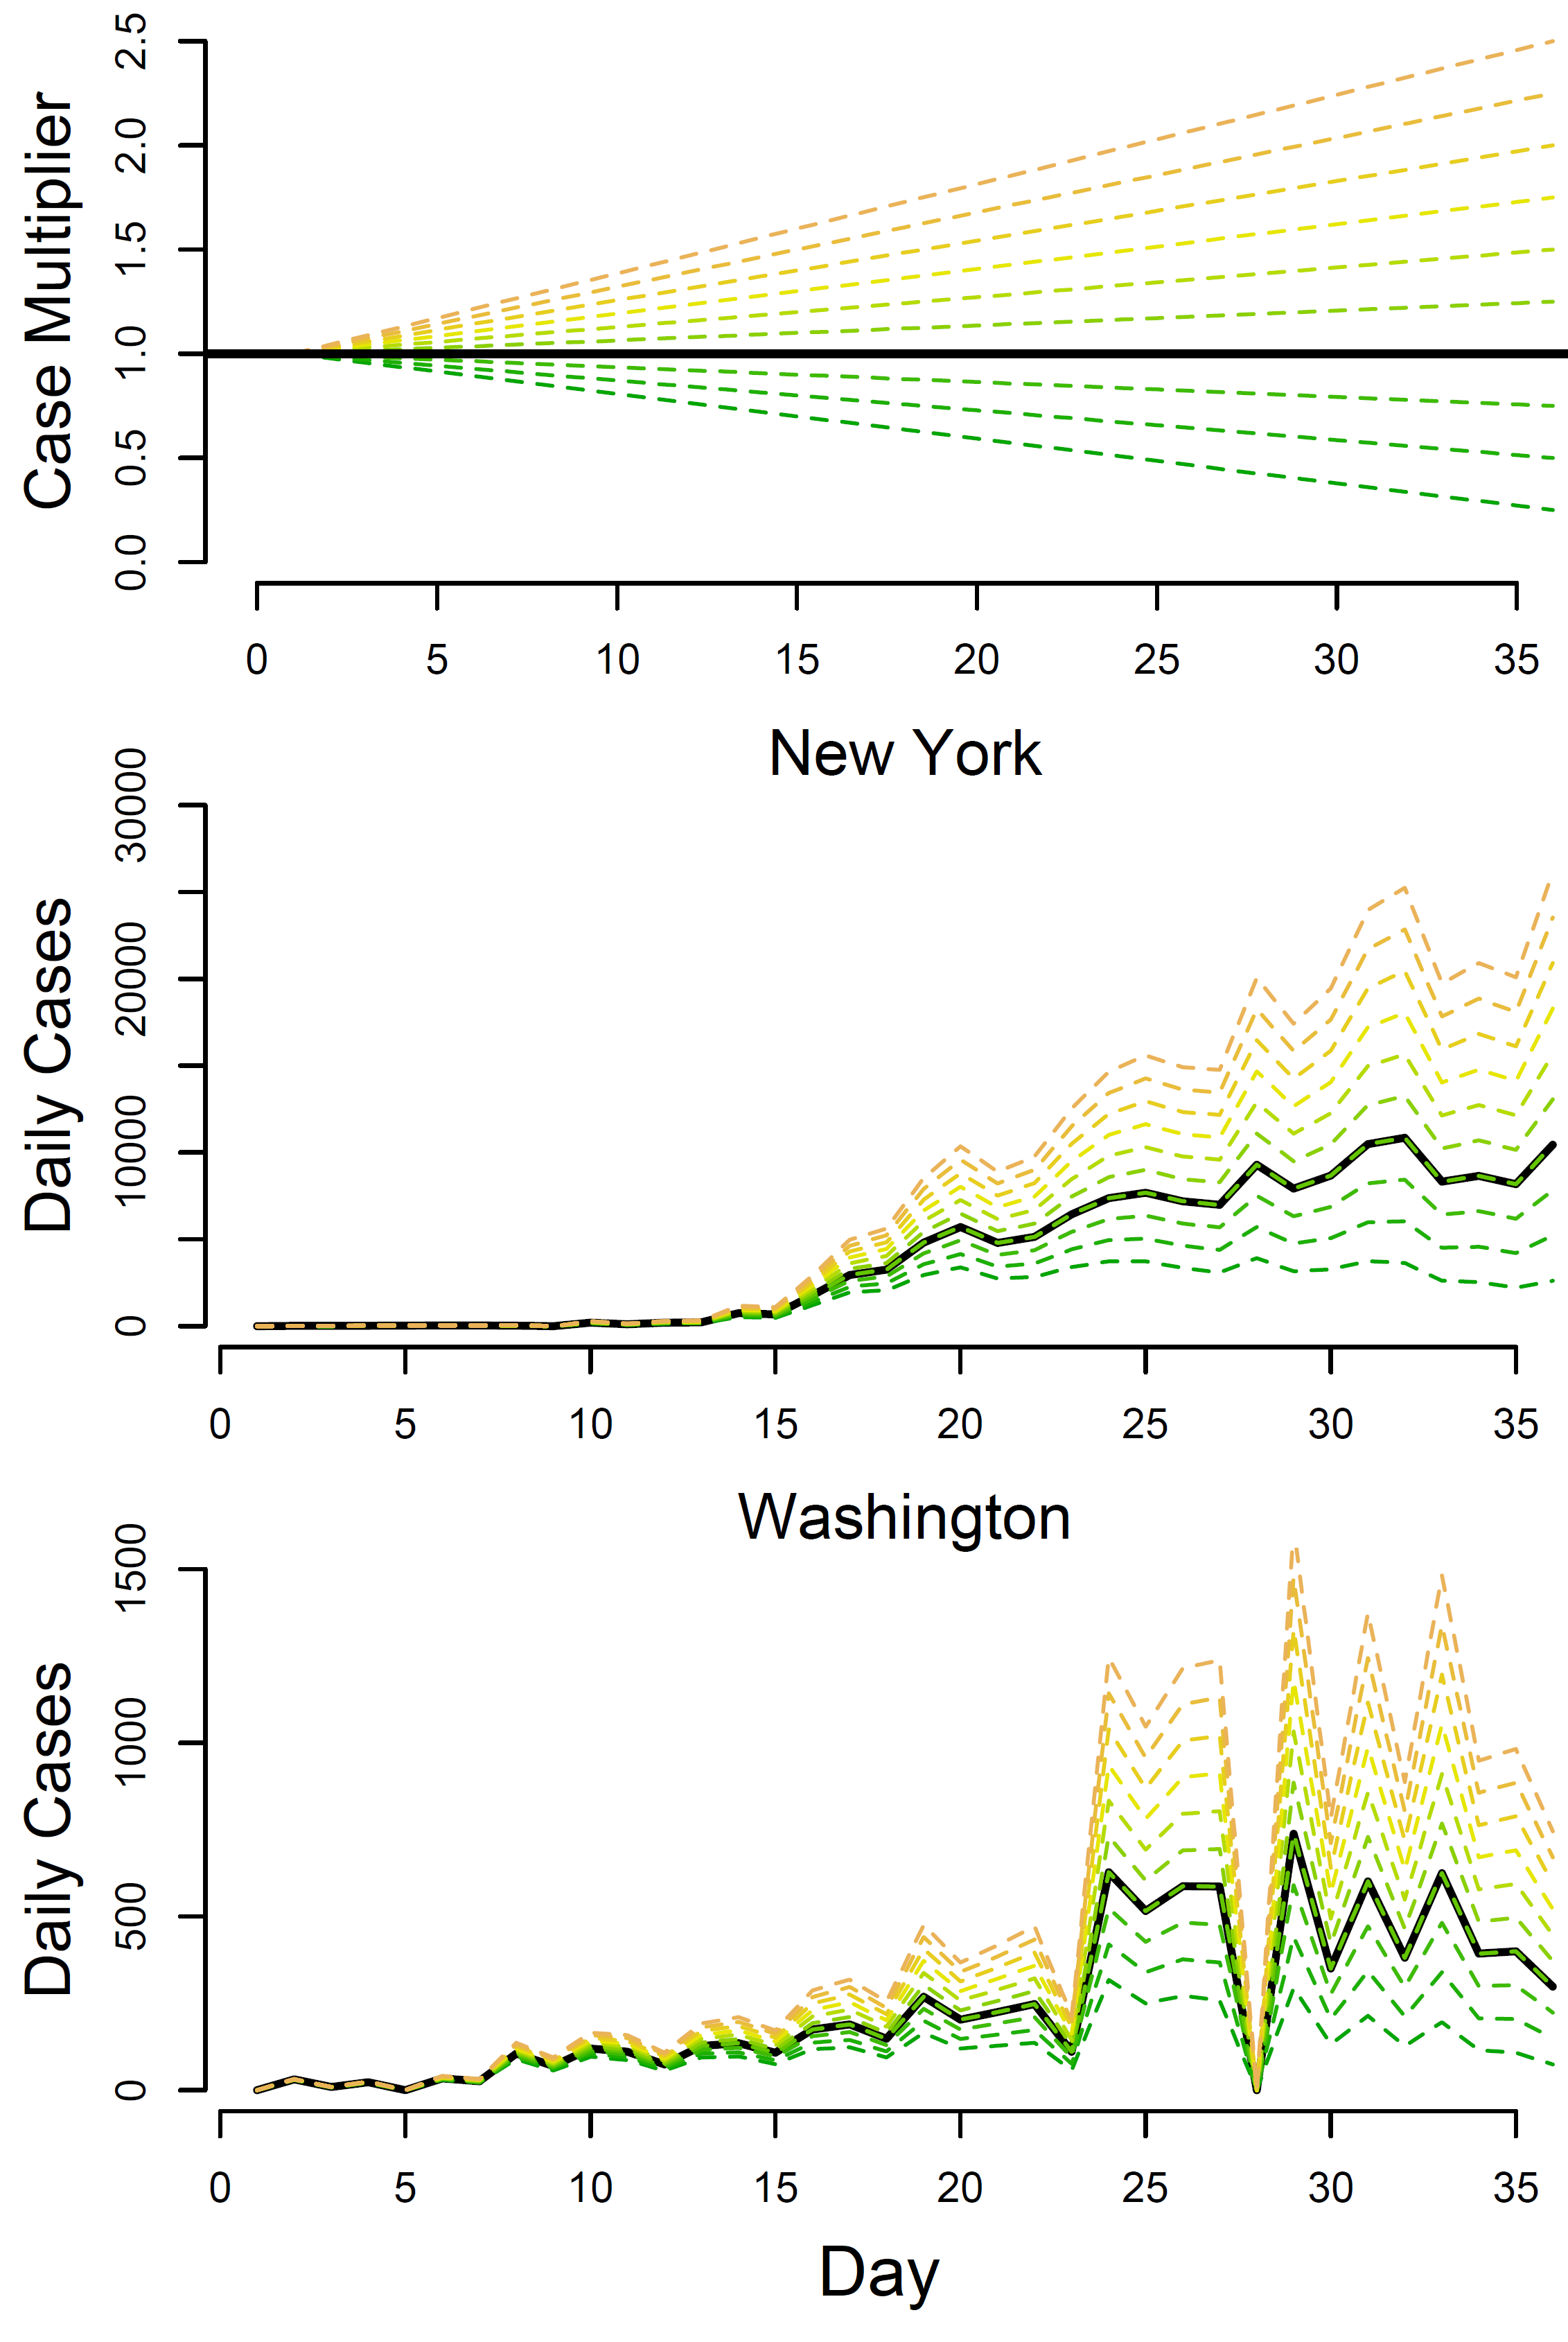
\includegraphics[width=10cm]{cases_multilpier.png}
\caption{}
\label{fig:bends}
\end{figure} 

\begin{figure}
\centering
\hspace*{0cm}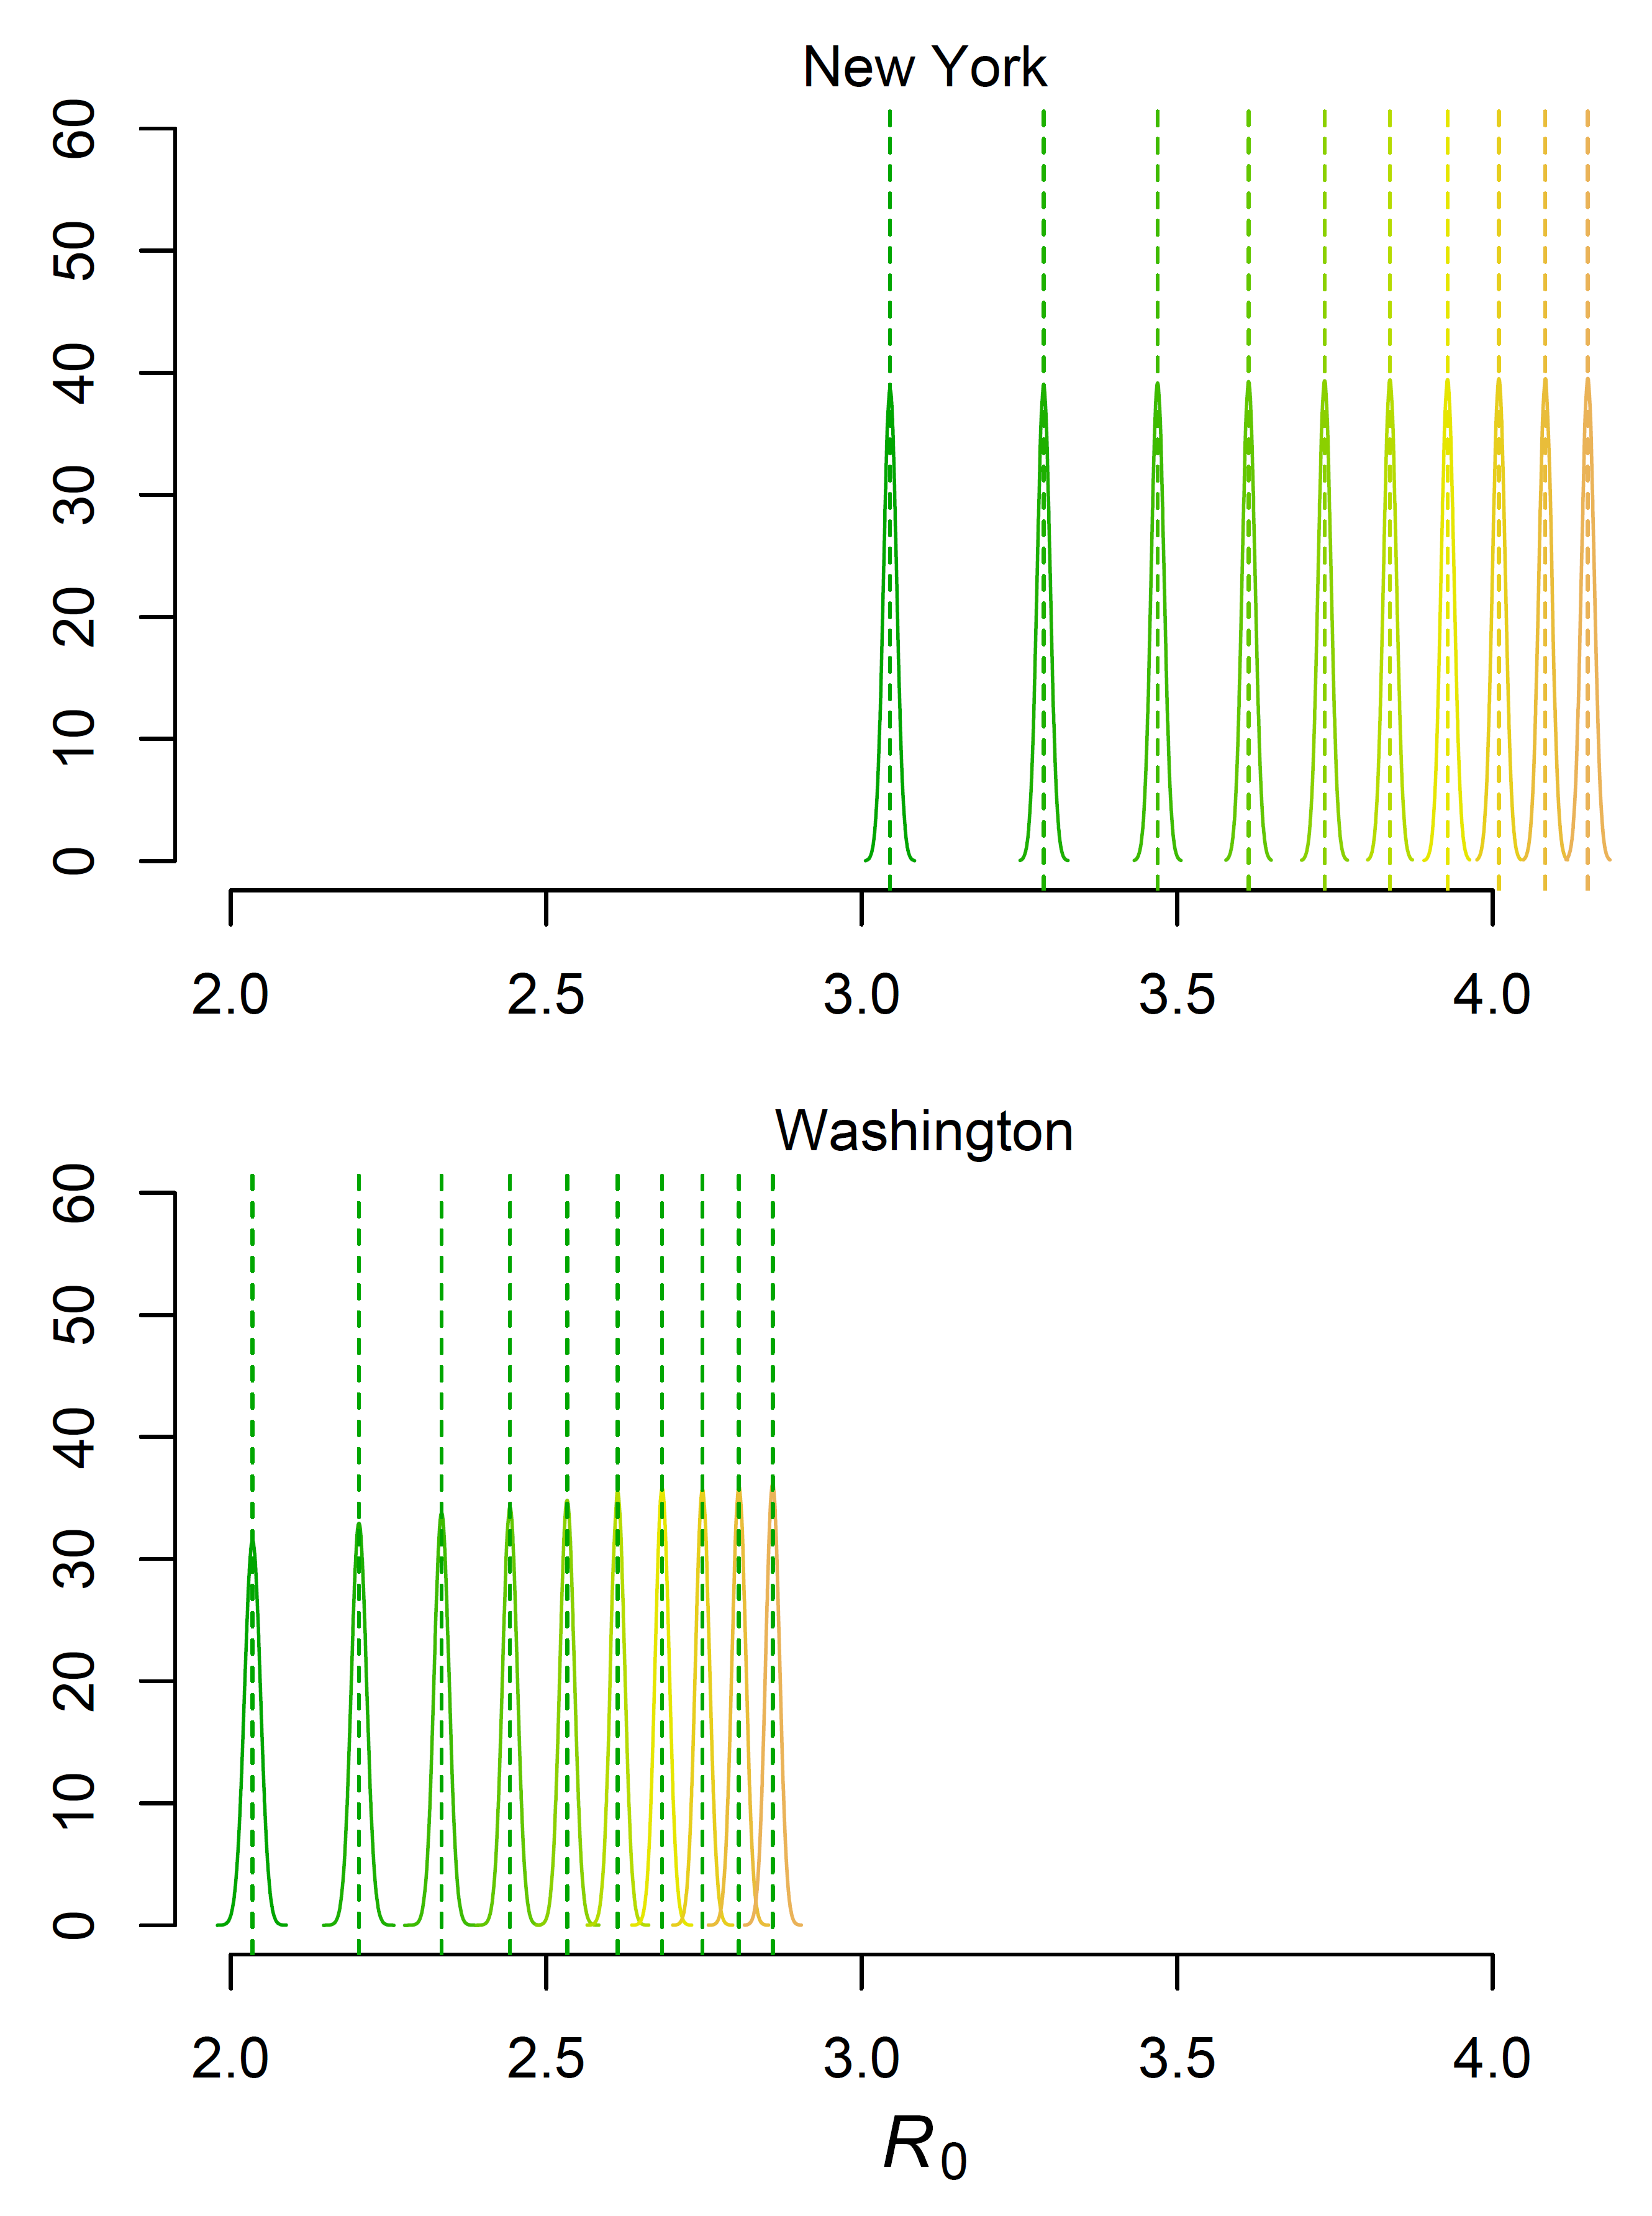
\includegraphics[width=12cm]{posteriors.png}
\caption{}
\label{fig:bends}
\end{figure} 

\begin{figure}
\centering
\hspace*{0cm}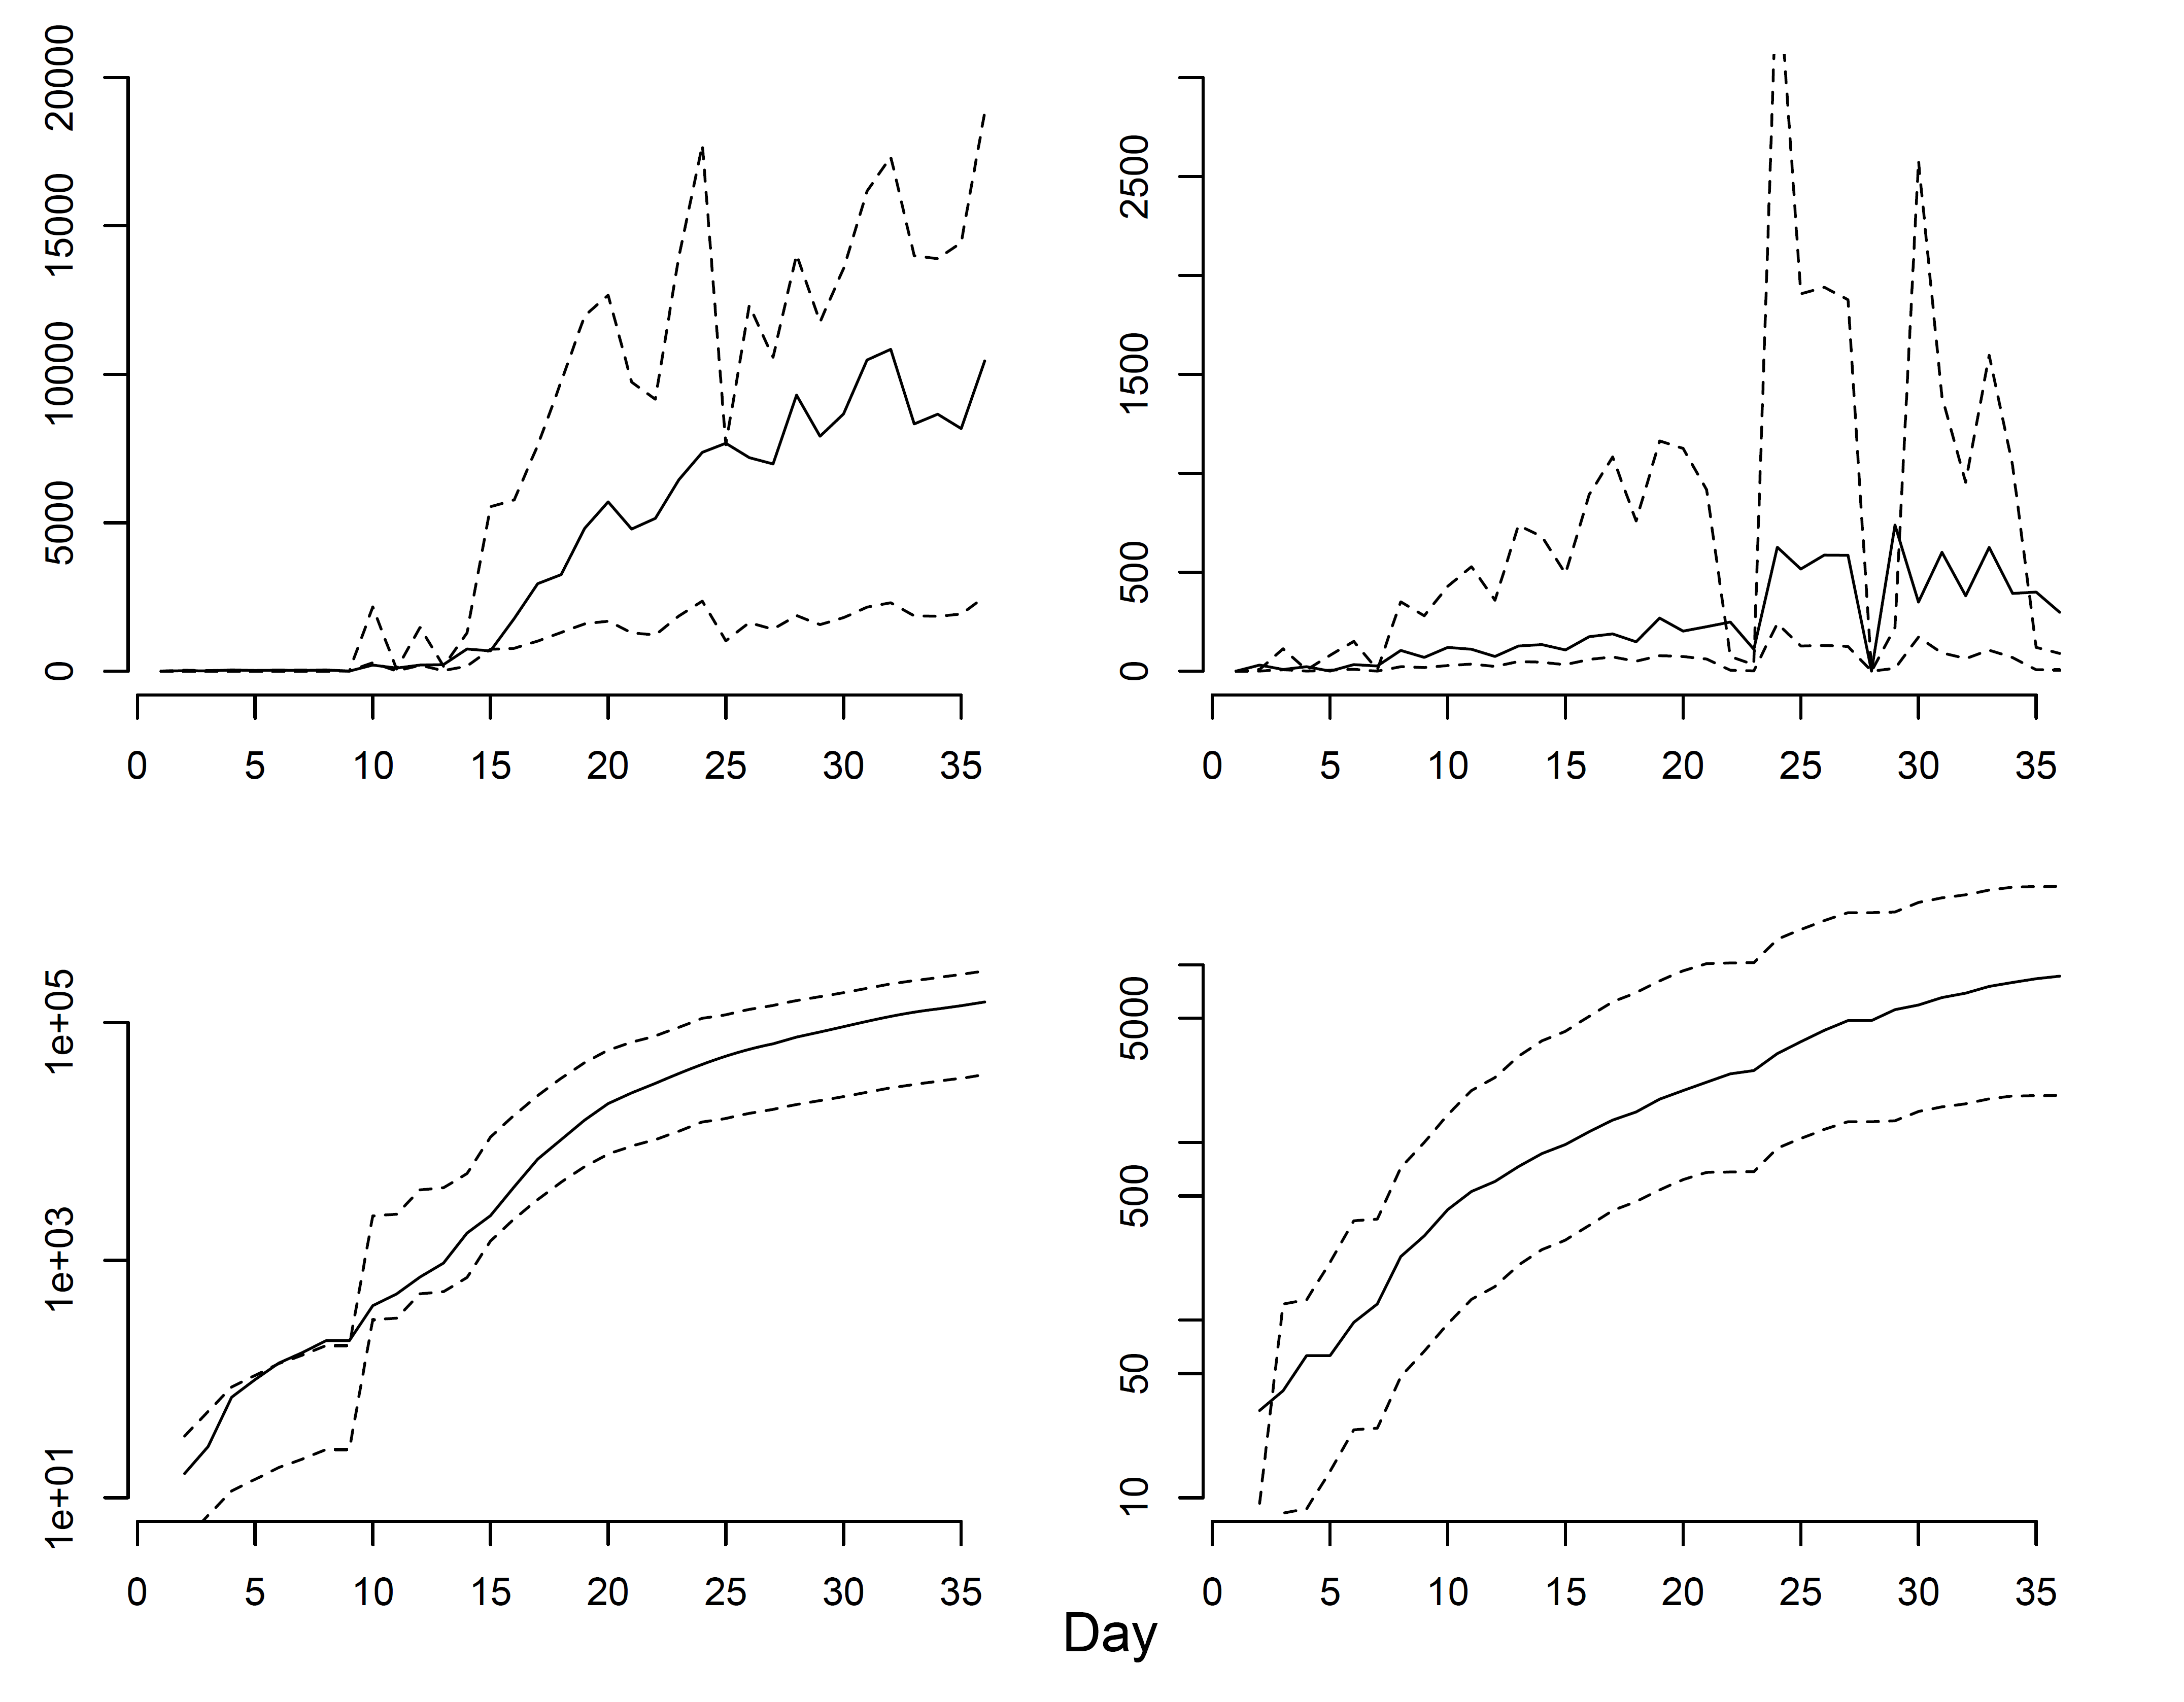
\includegraphics[width=14cm]{NY_WA_up_dn.png}
\caption{}
\label{fig:bends}
\end{figure} 

\begin{figure}
\centering
\hspace*{0cm}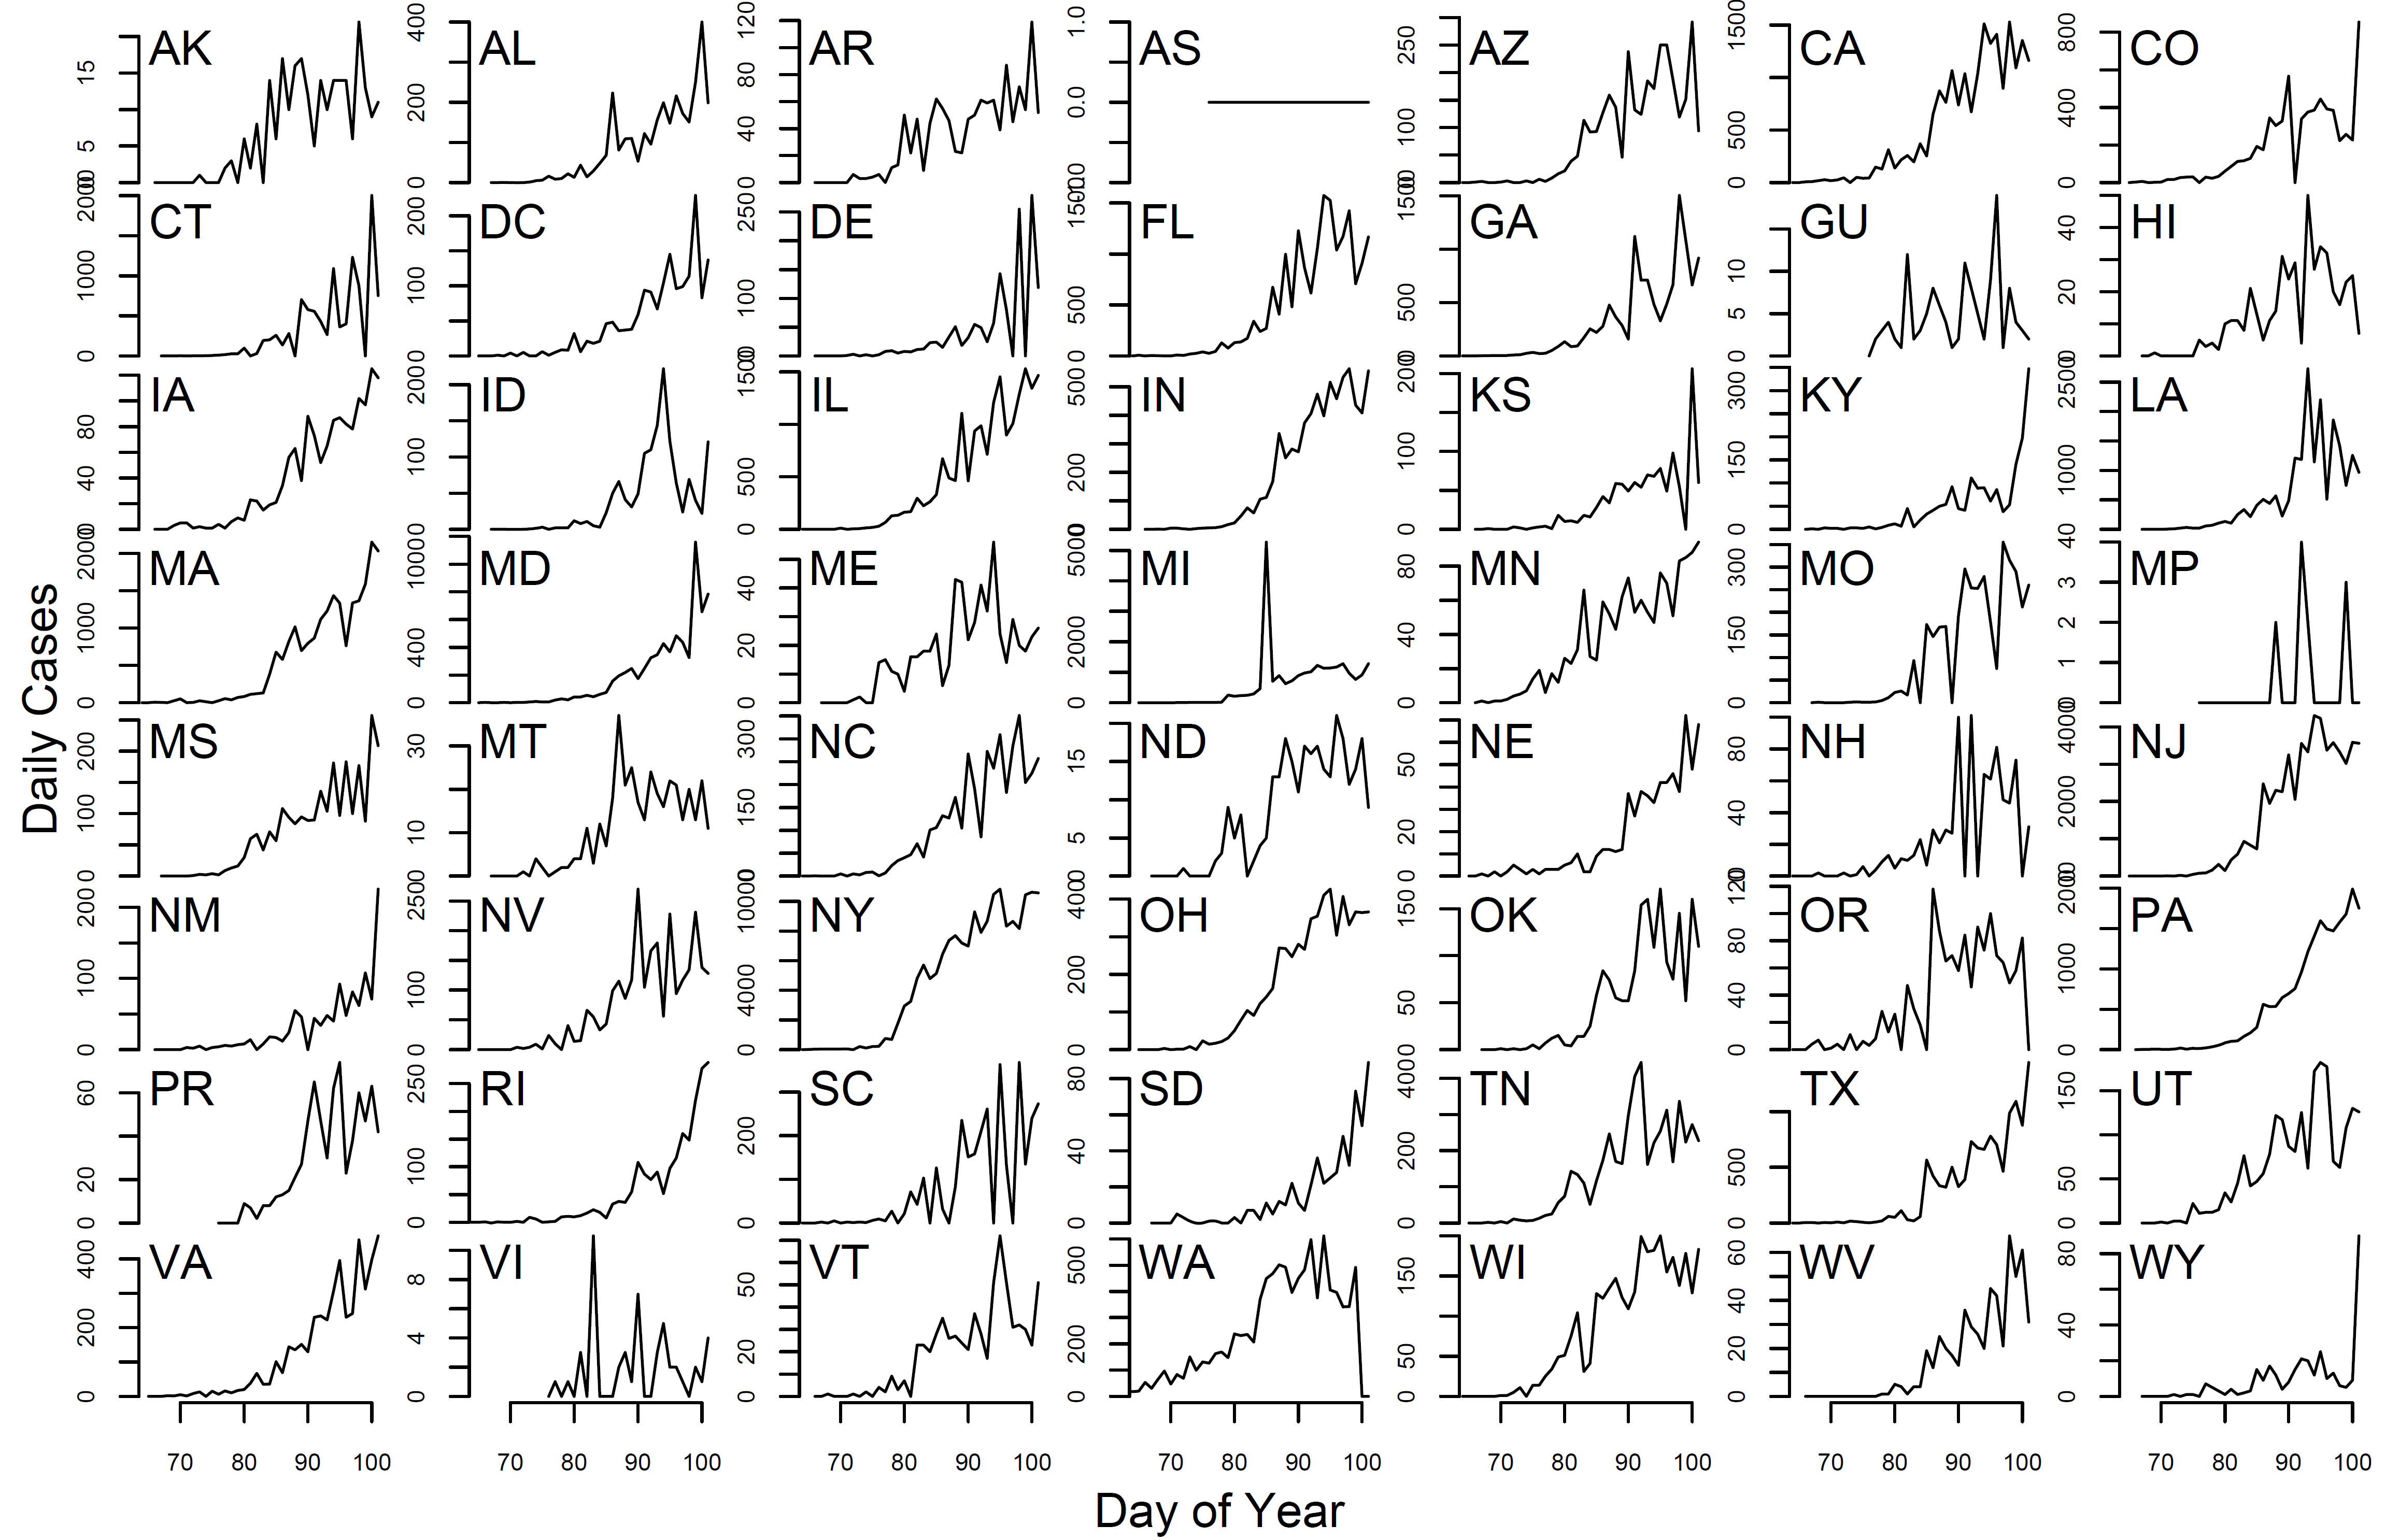
\includegraphics[width=16cm]{states_daily_cases.png}
\caption{}
\label{fig:bends}
\end{figure} 

\begin{figure}
\centering
\hspace*{0cm}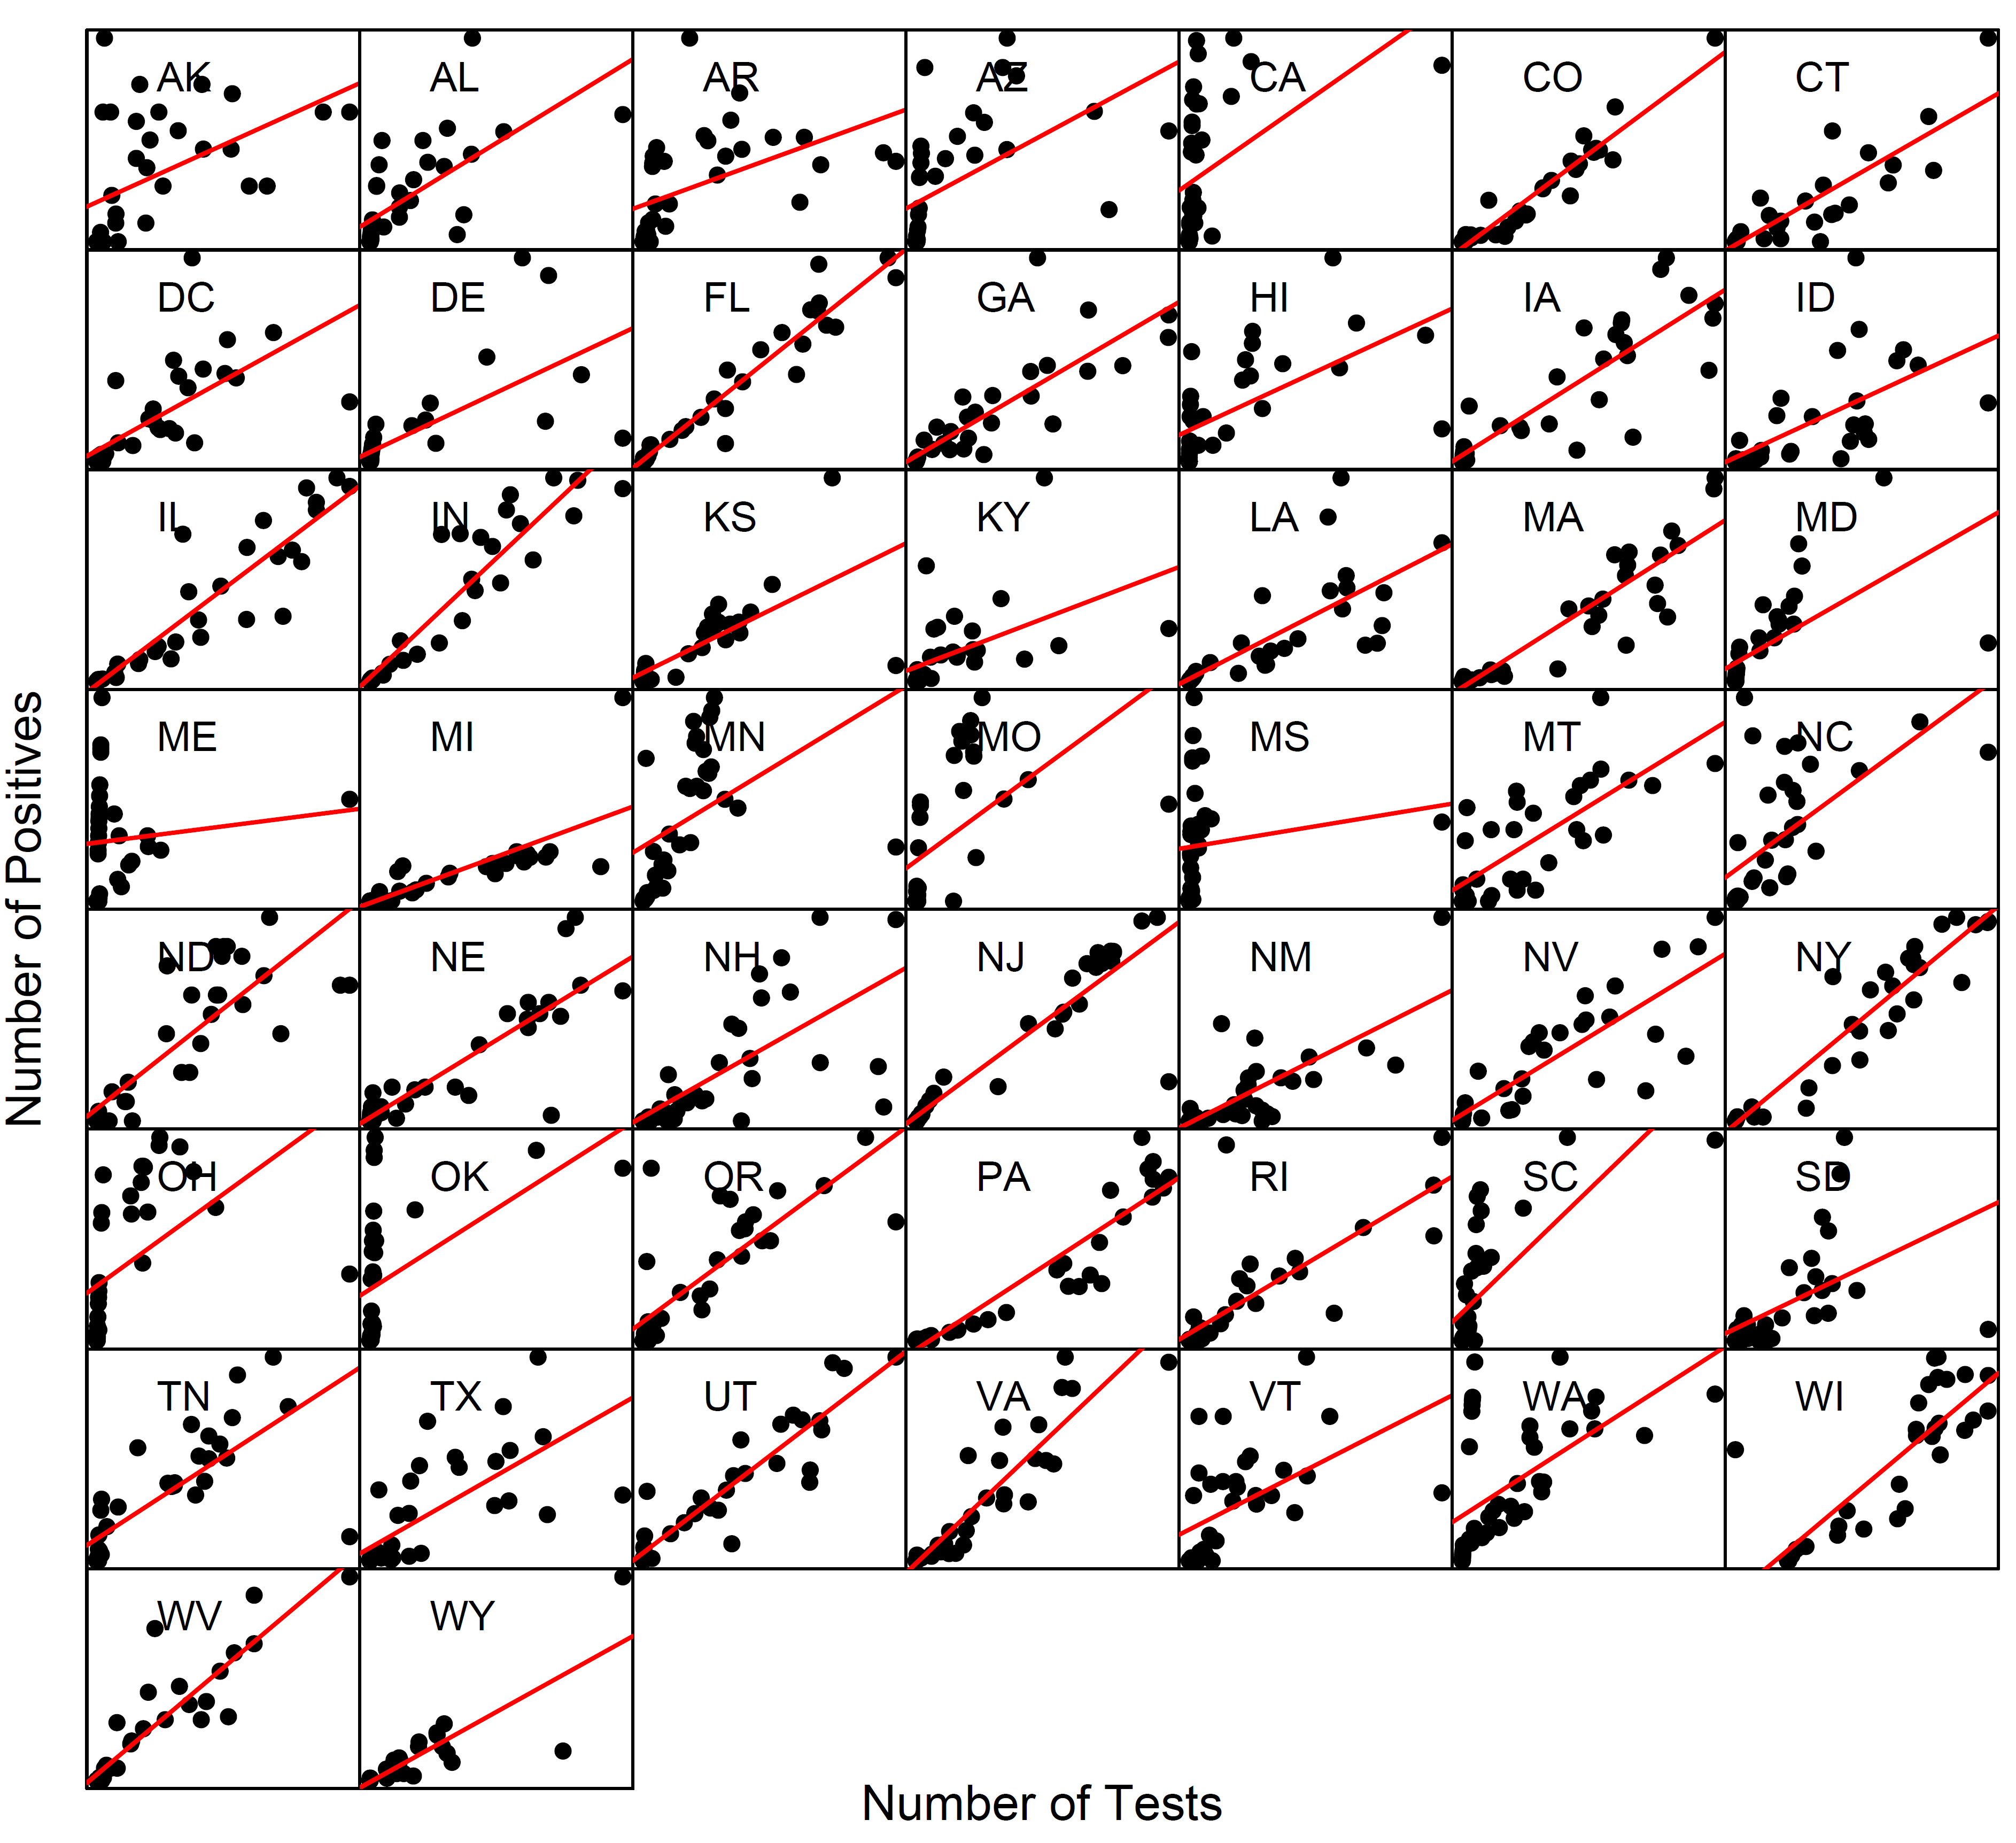
\includegraphics[width=14cm]{number_of_tests_vs_positives.png}
\caption{}
\label{fig:bends}
\end{figure} 

\begin{figure}
\centering
\hspace*{0cm}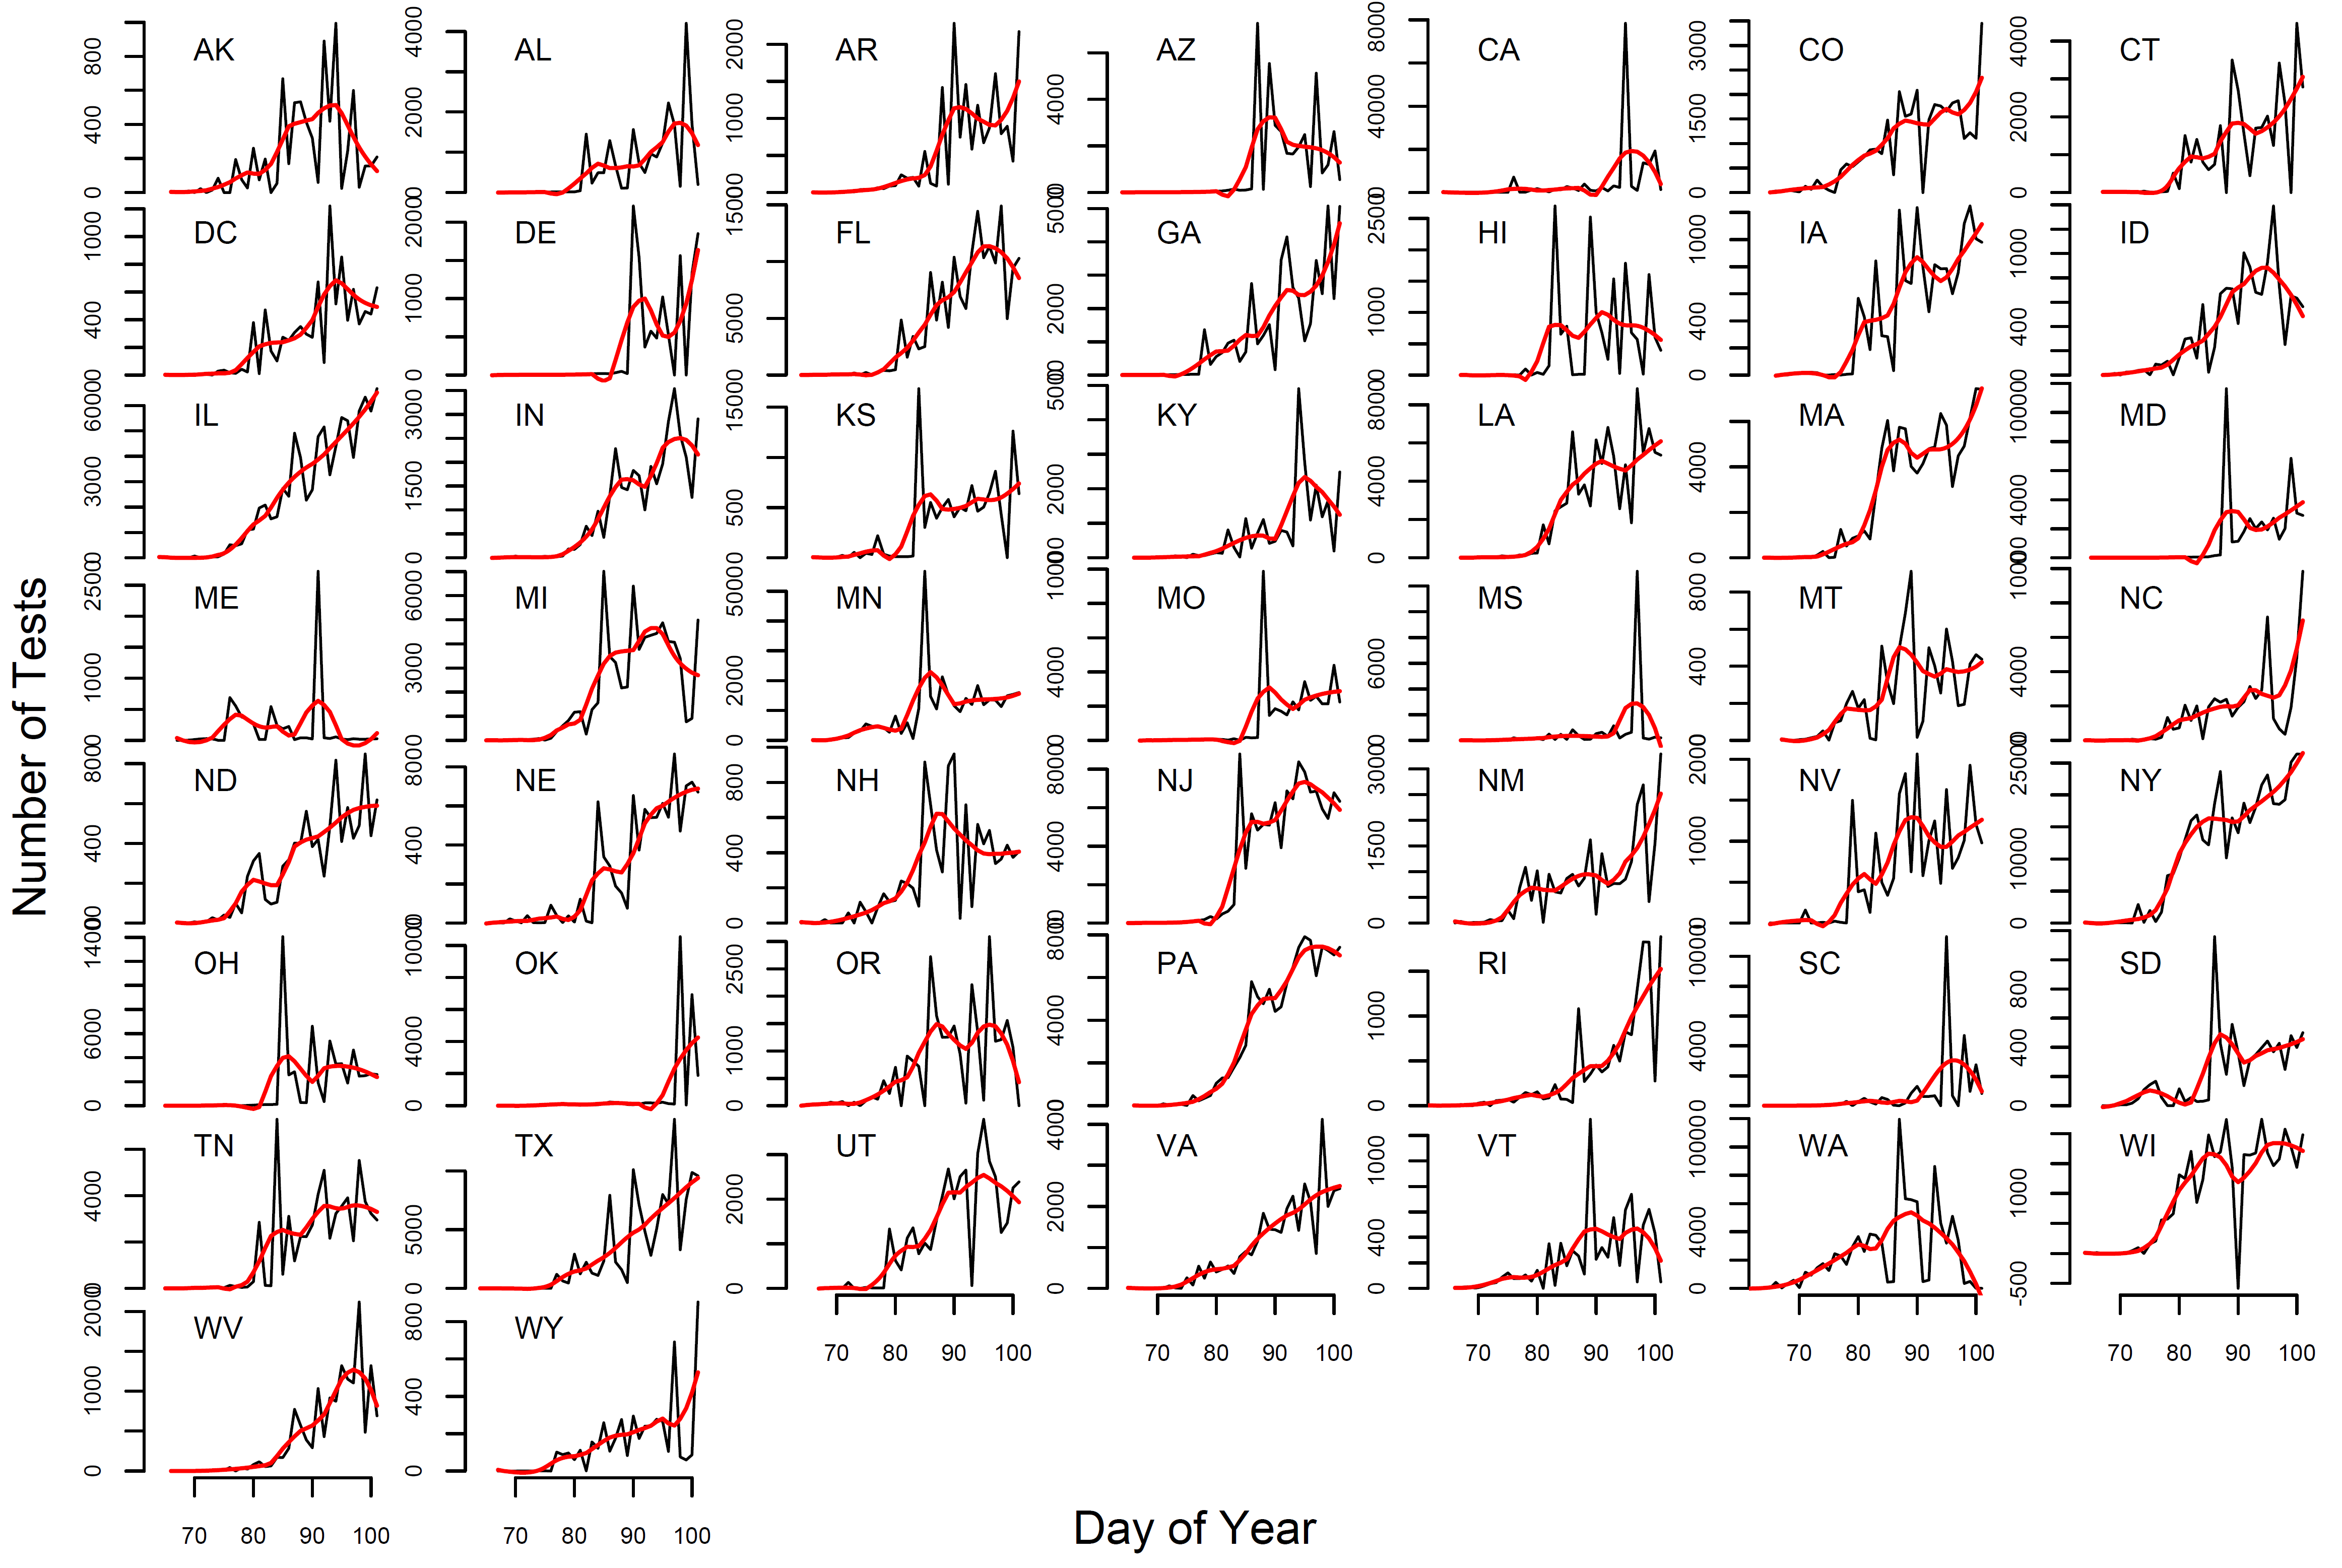
\includegraphics[width=16cm]{number_of_tests_span04.png}
\caption{}
\label{fig:bends}
\end{figure} 

\begin{figure}
\centering
\hspace*{0cm}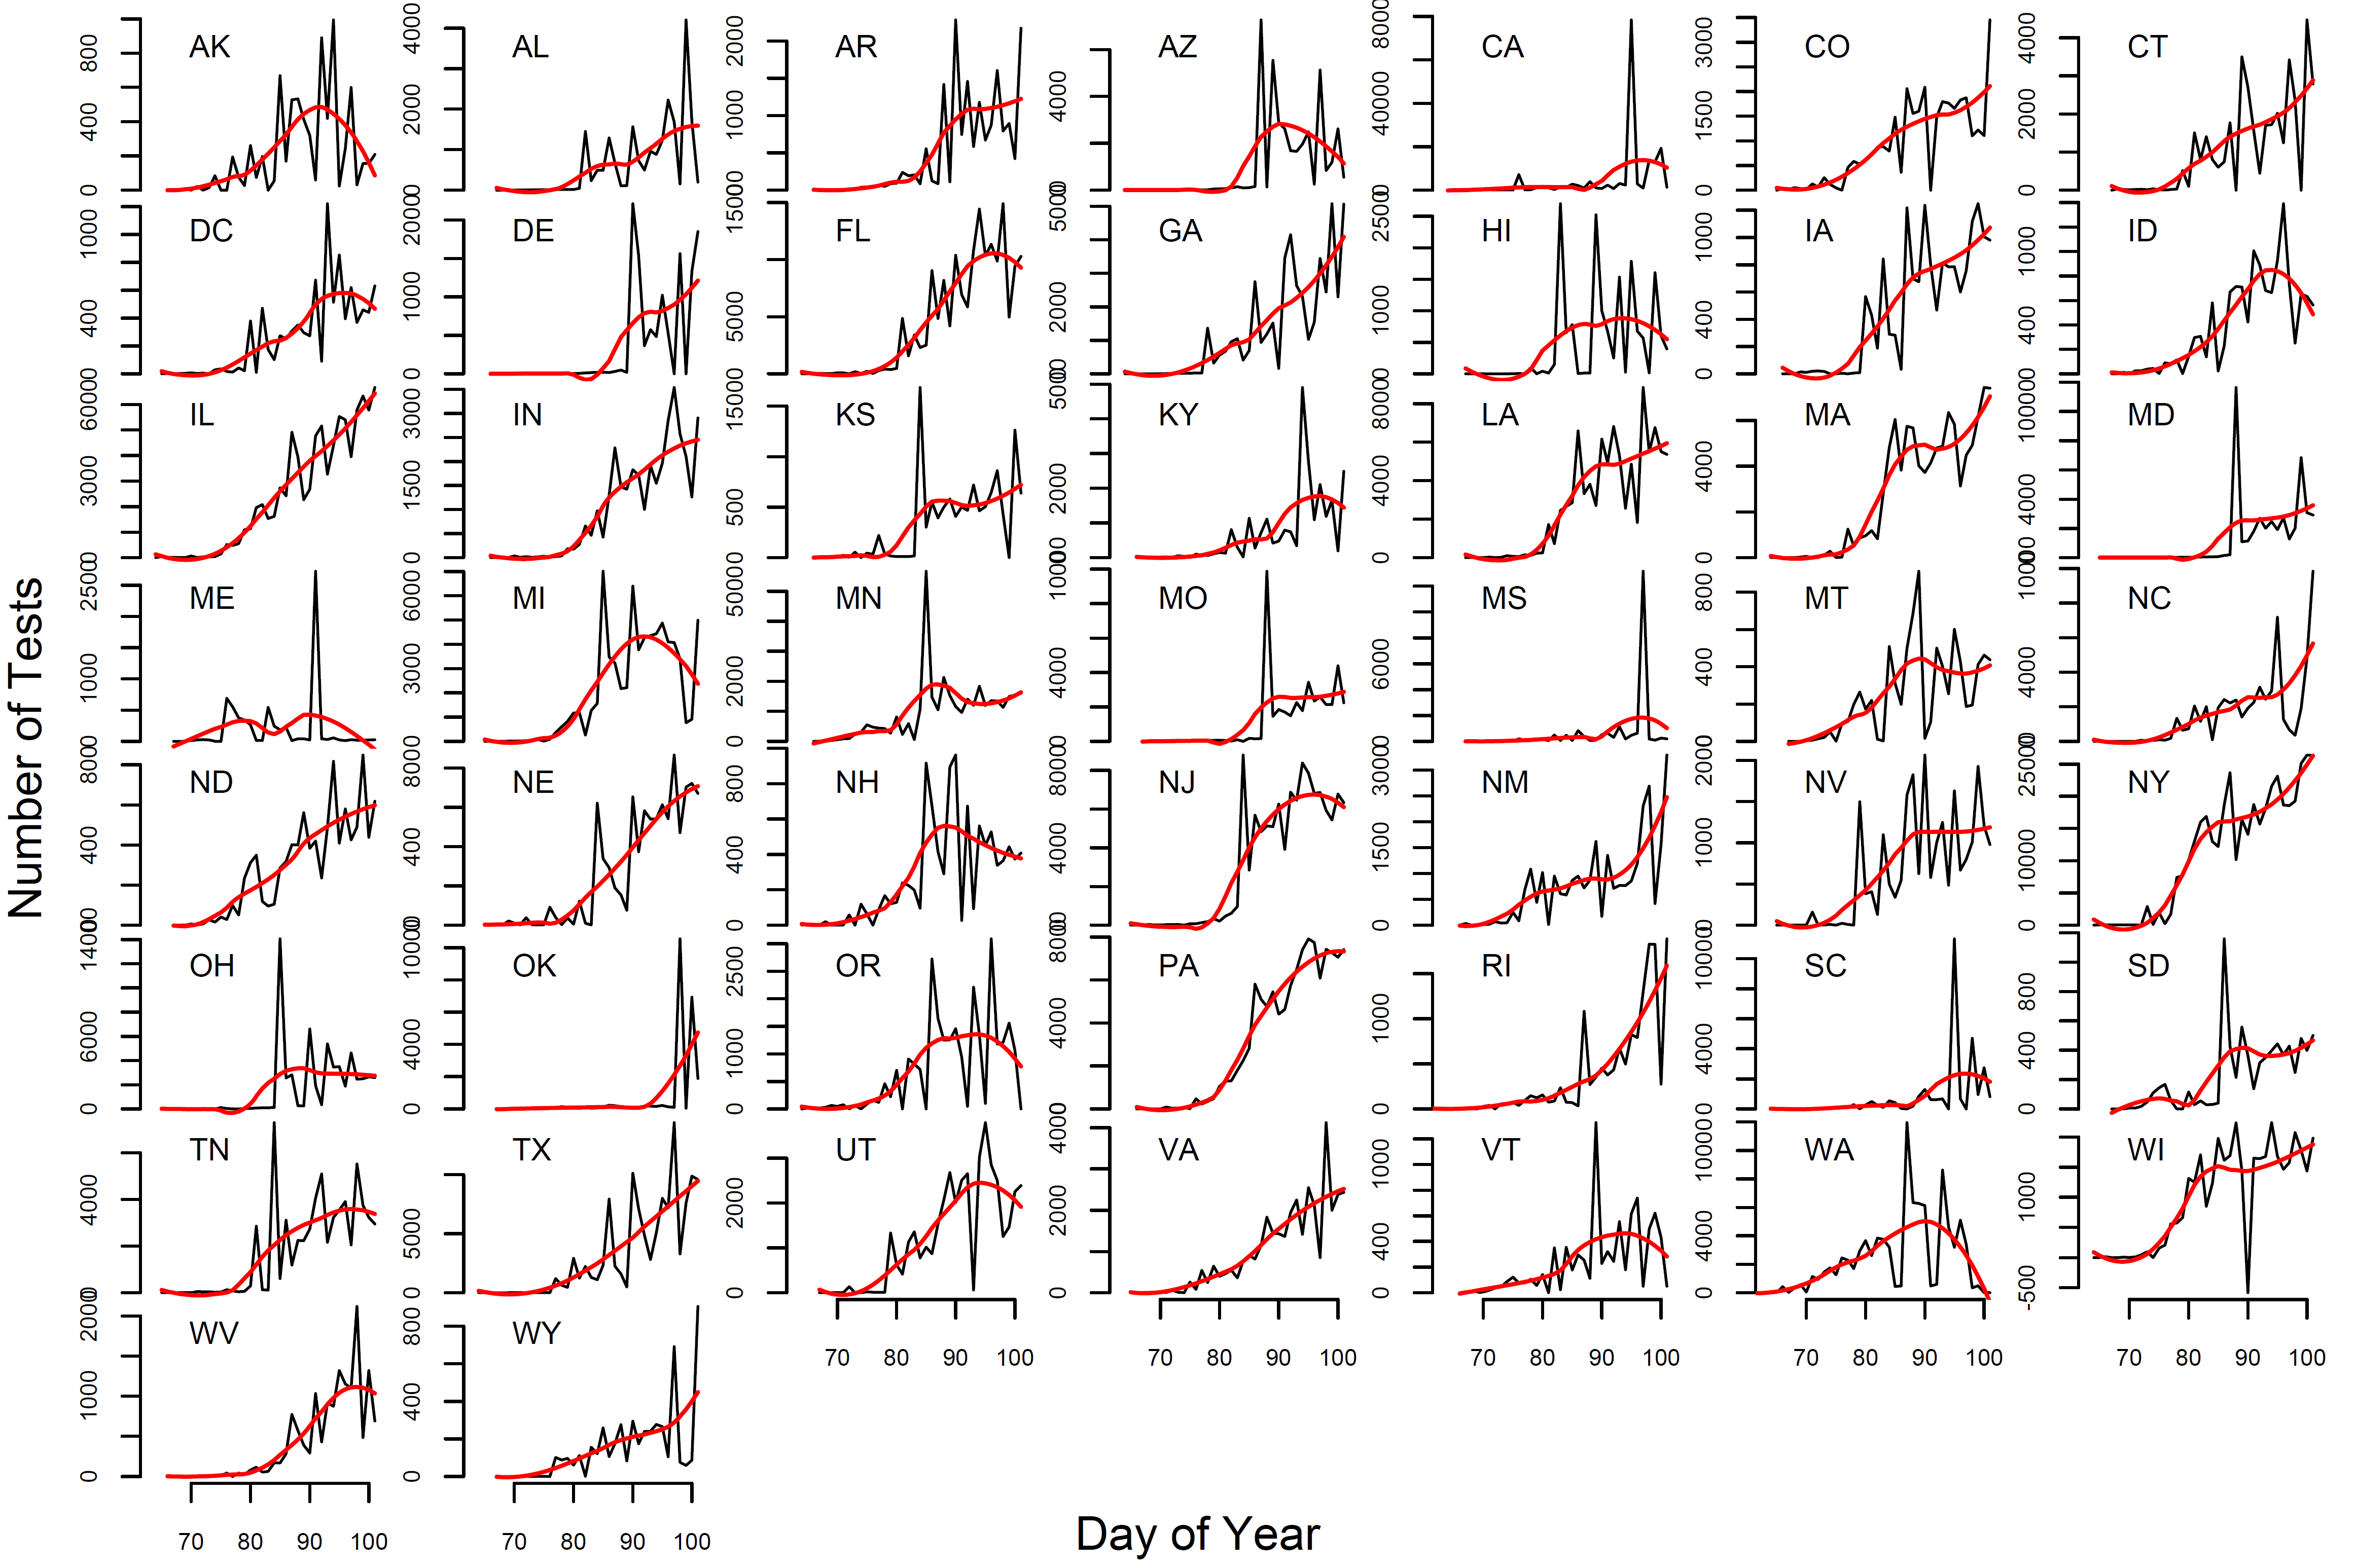
\includegraphics[width=16cm]{number_of_tests_span06.png}
\caption{}
\label{fig:bends}
\end{figure} 

\begin{figure}
\centering
\hspace*{0cm}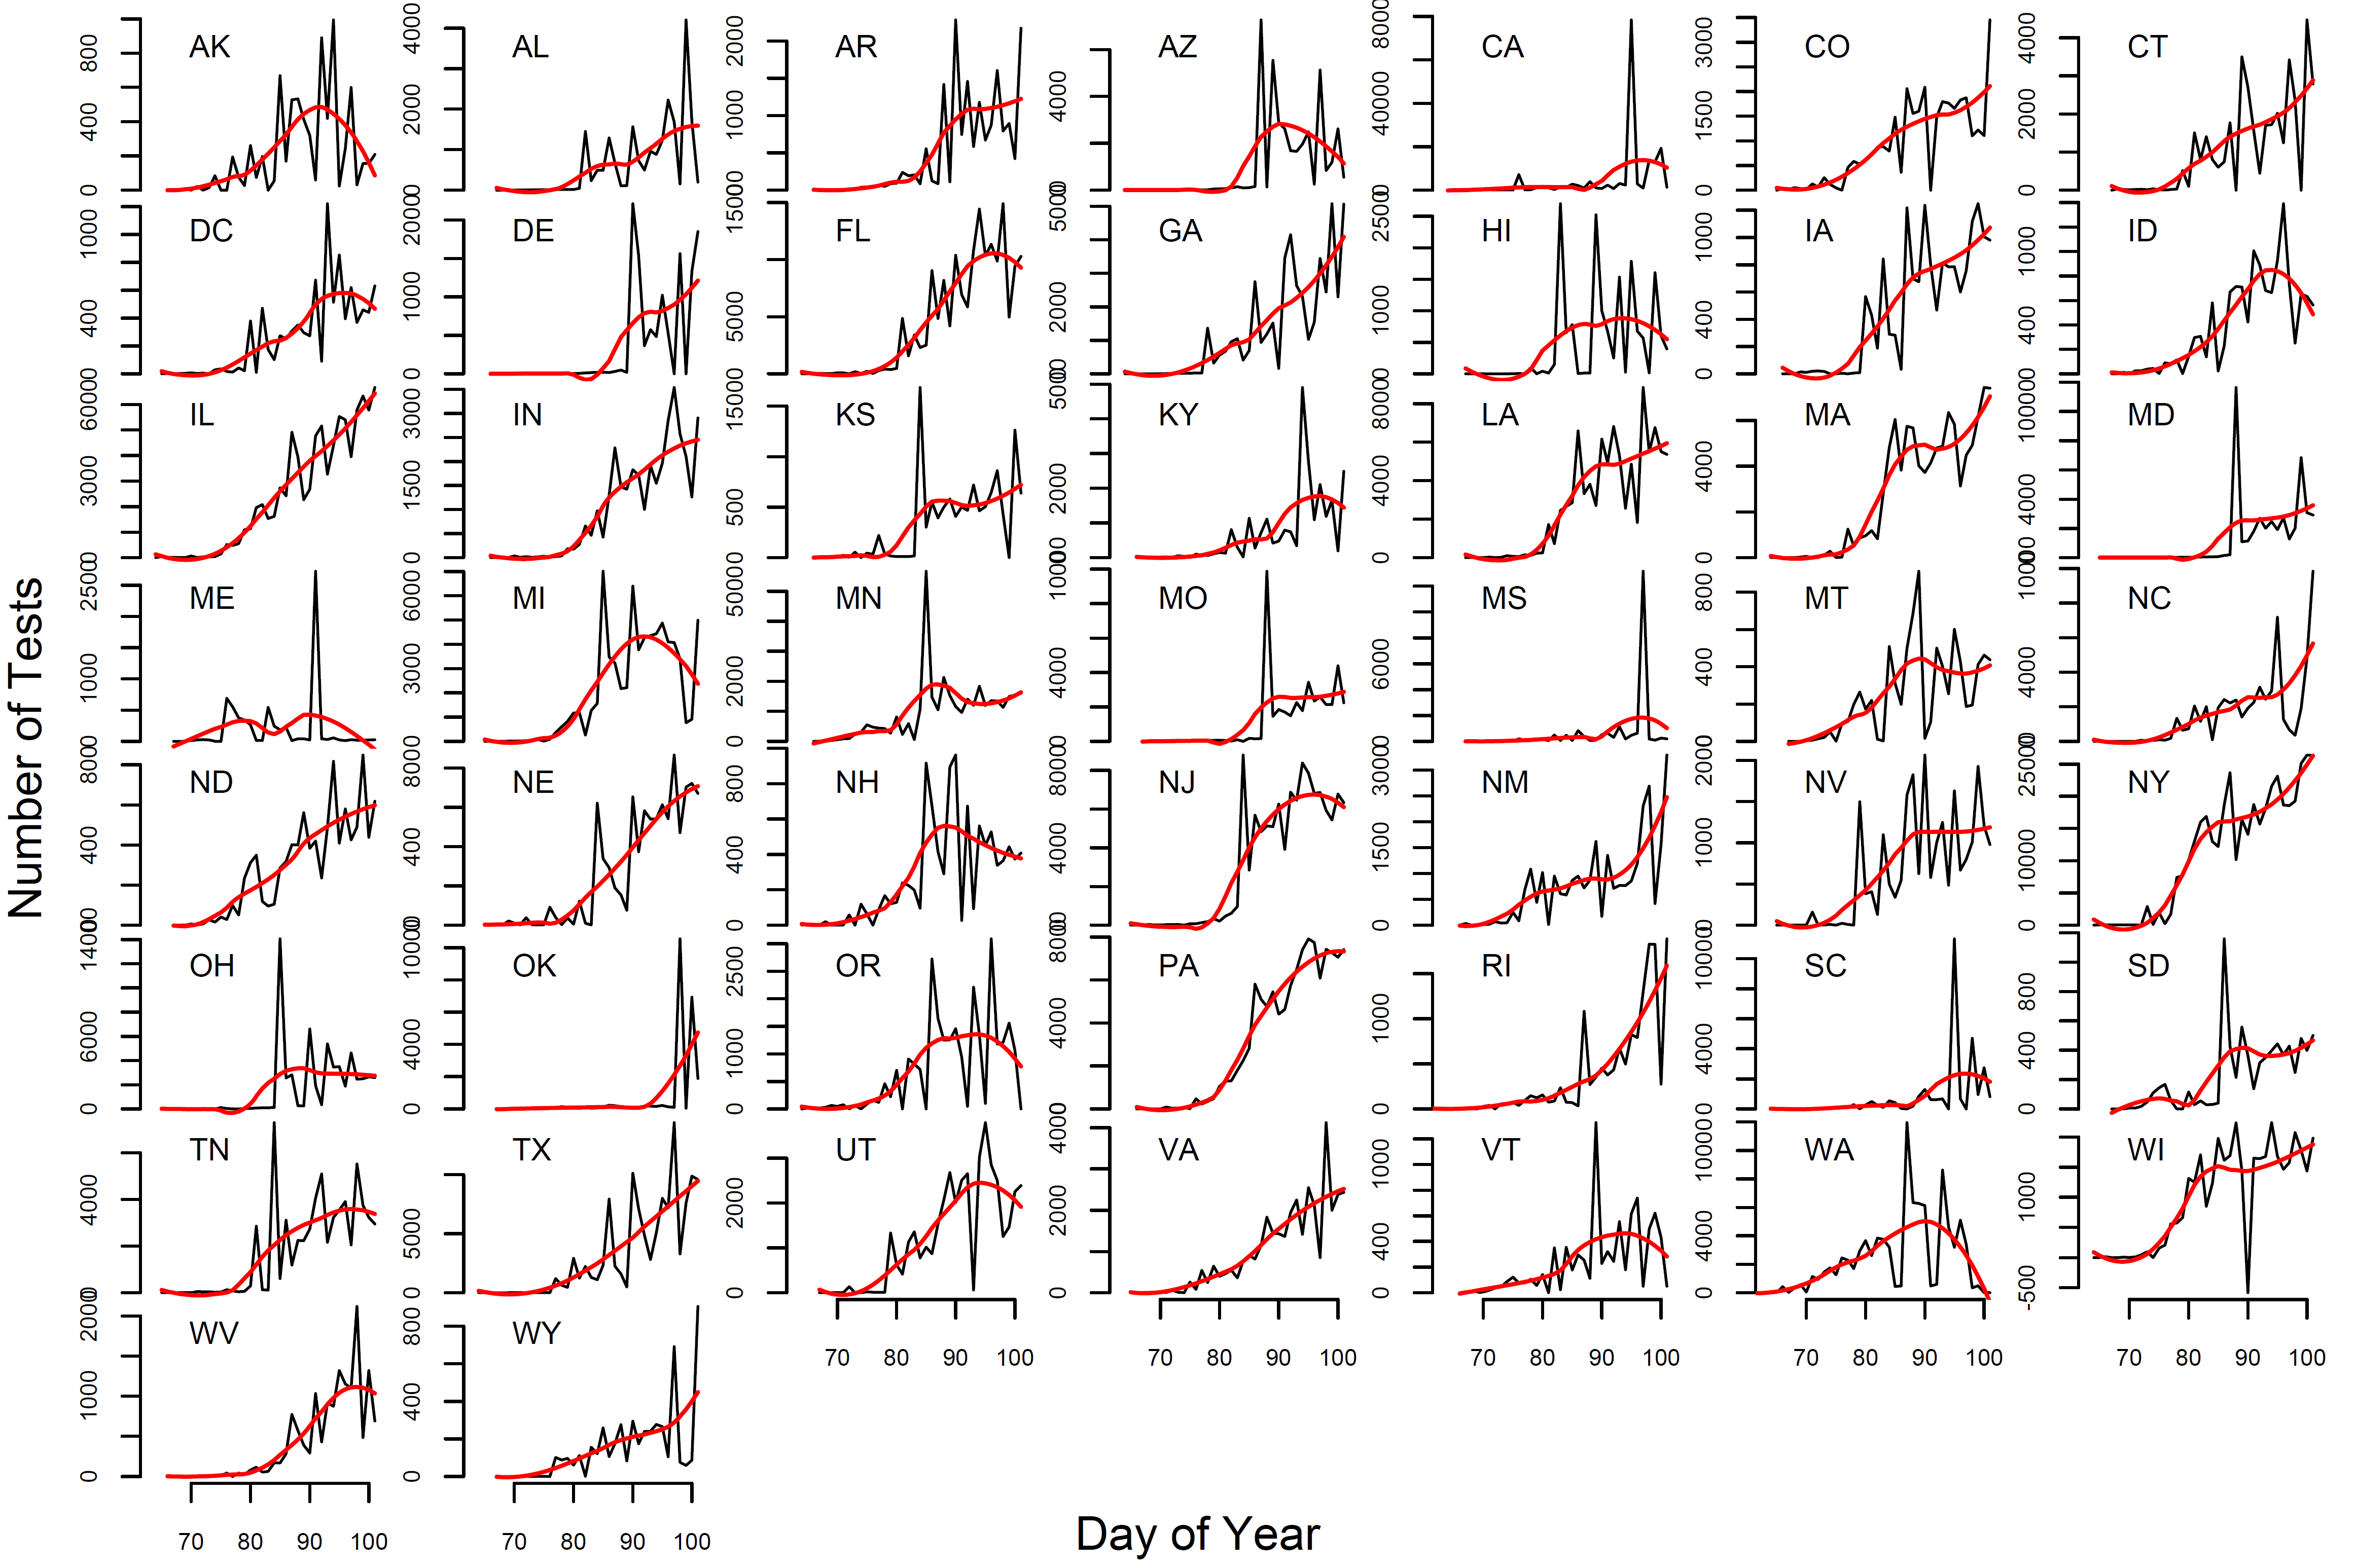
\includegraphics[width=16cm]{number_of_tests_span06.png}
\caption{}
\label{fig:bends}
\end{figure} 

\begin{figure}
\centering
\hspace*{0cm}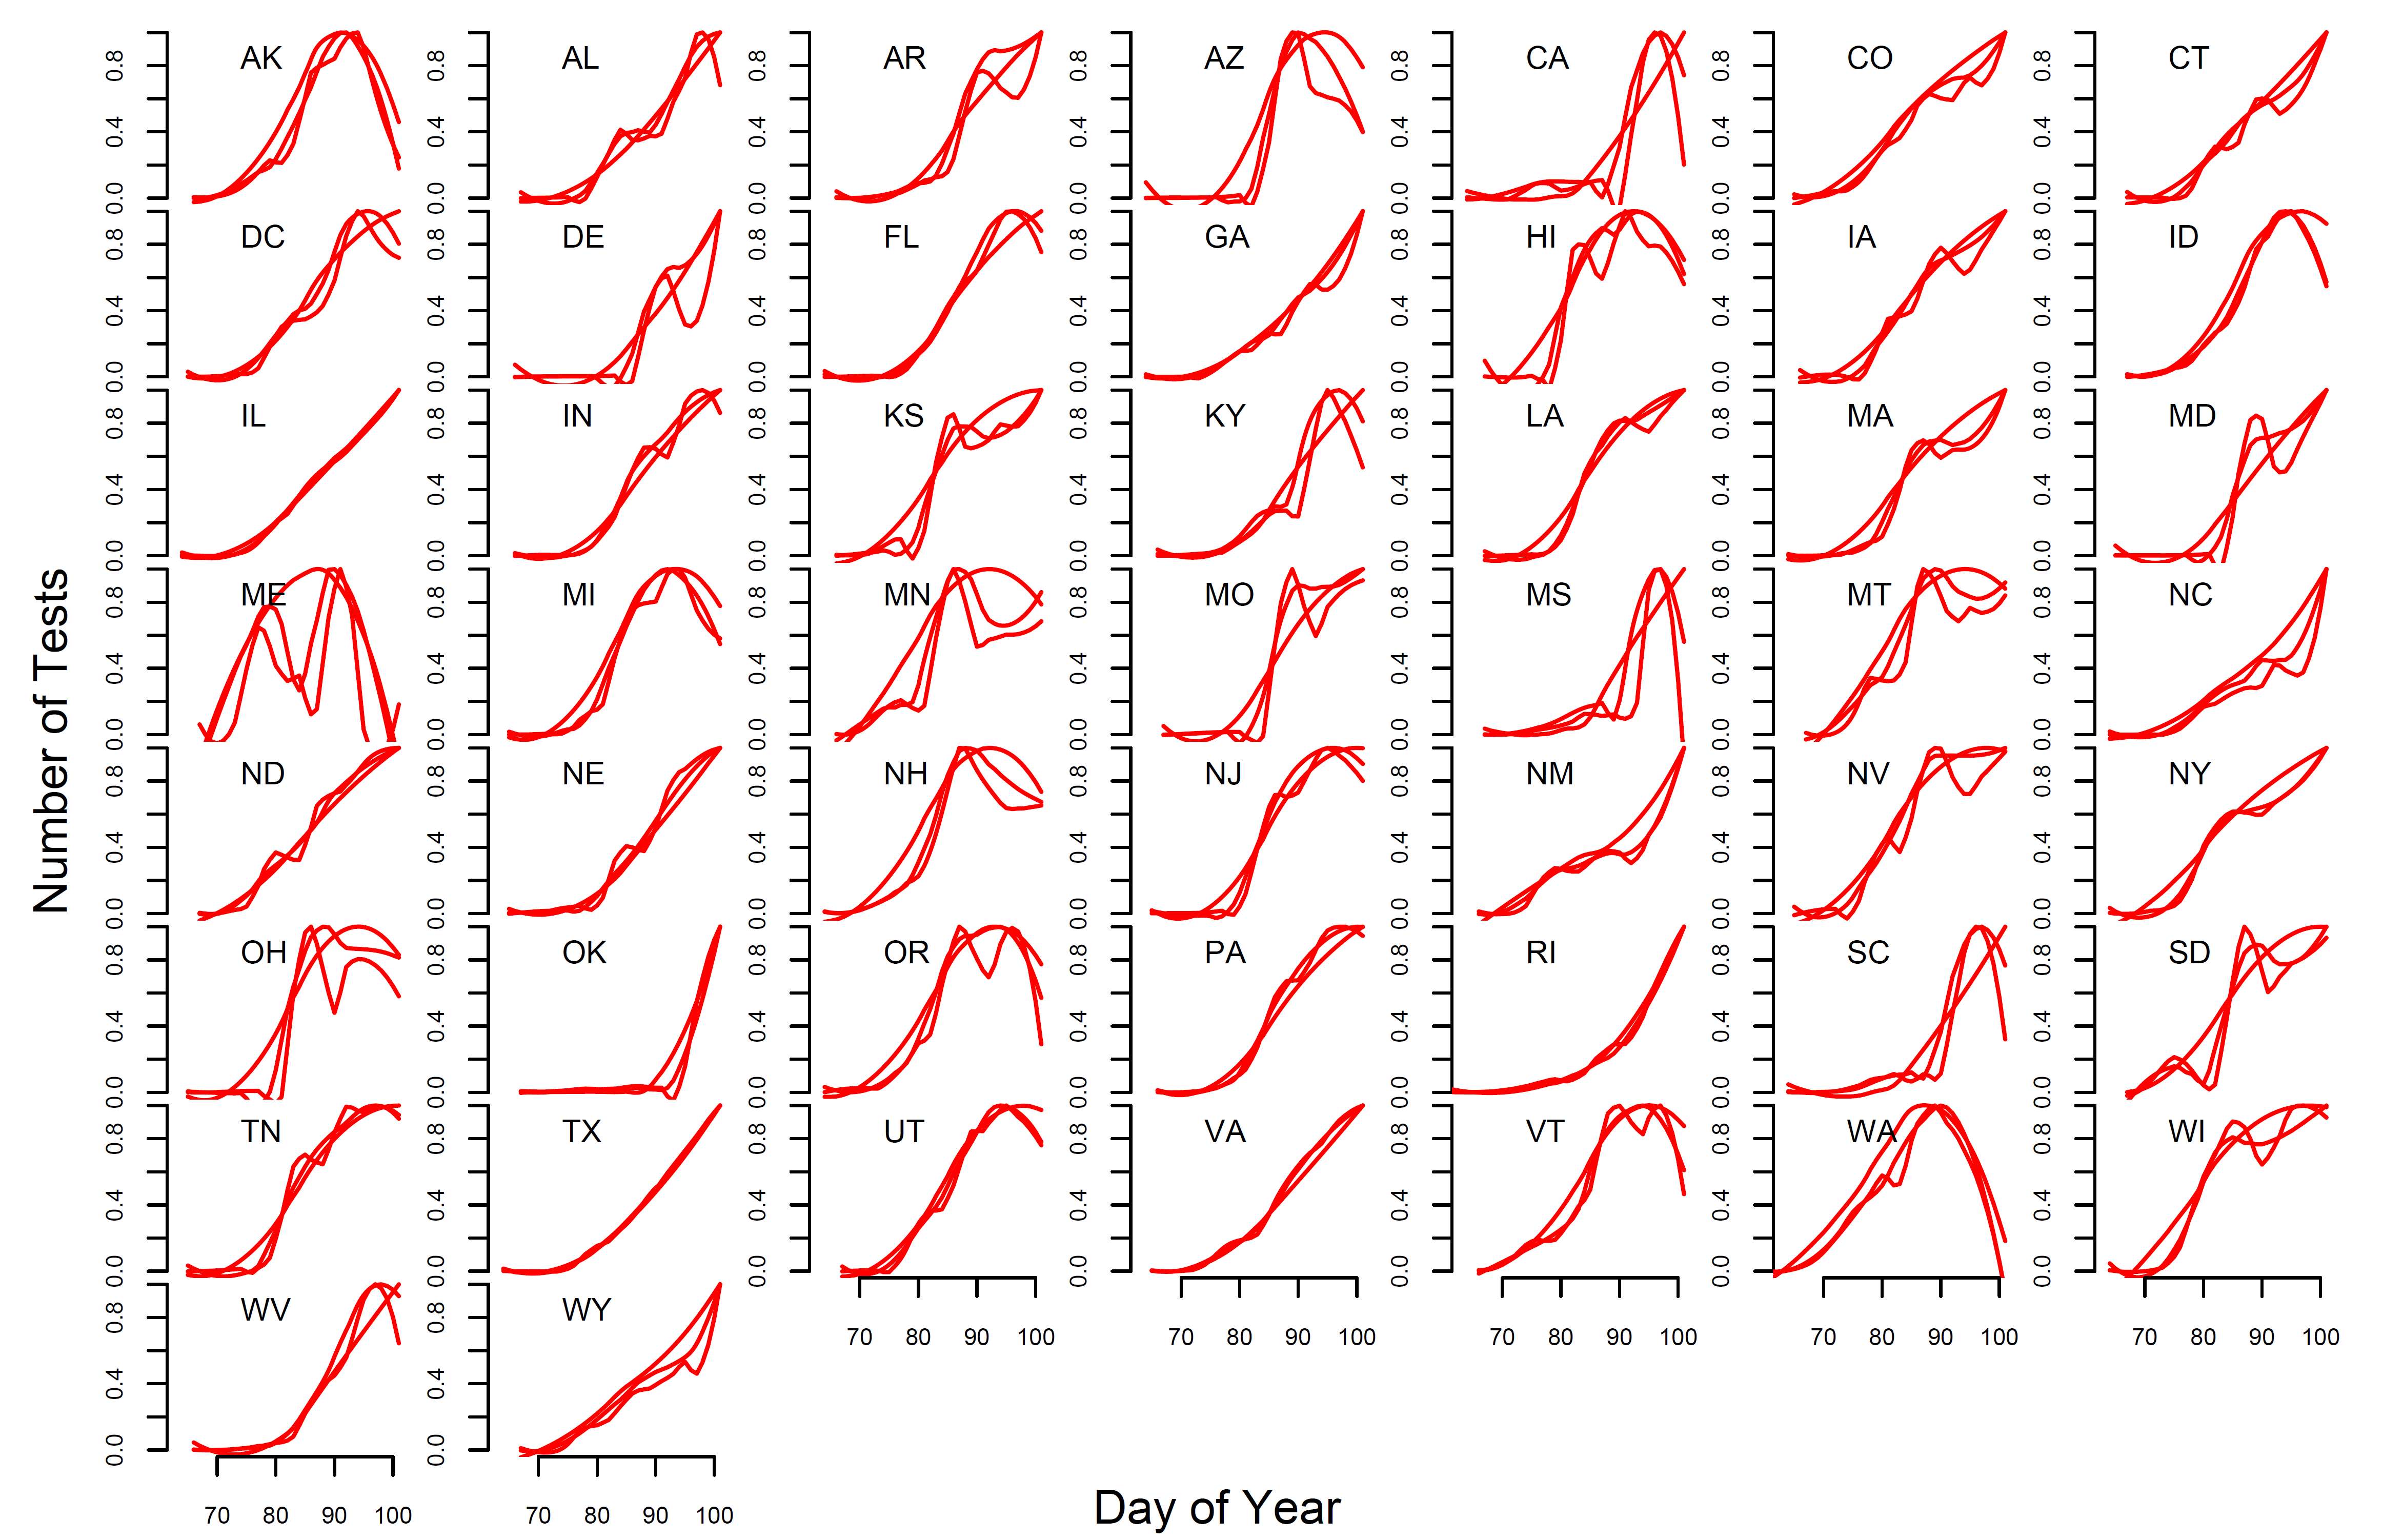
\includegraphics[width=16cm]{number_of_tests_factor_04_06_10.png}
\caption{}
\label{fig:bends}
\end{figure} 


\begin{figure}
\centering
\hspace*{0cm}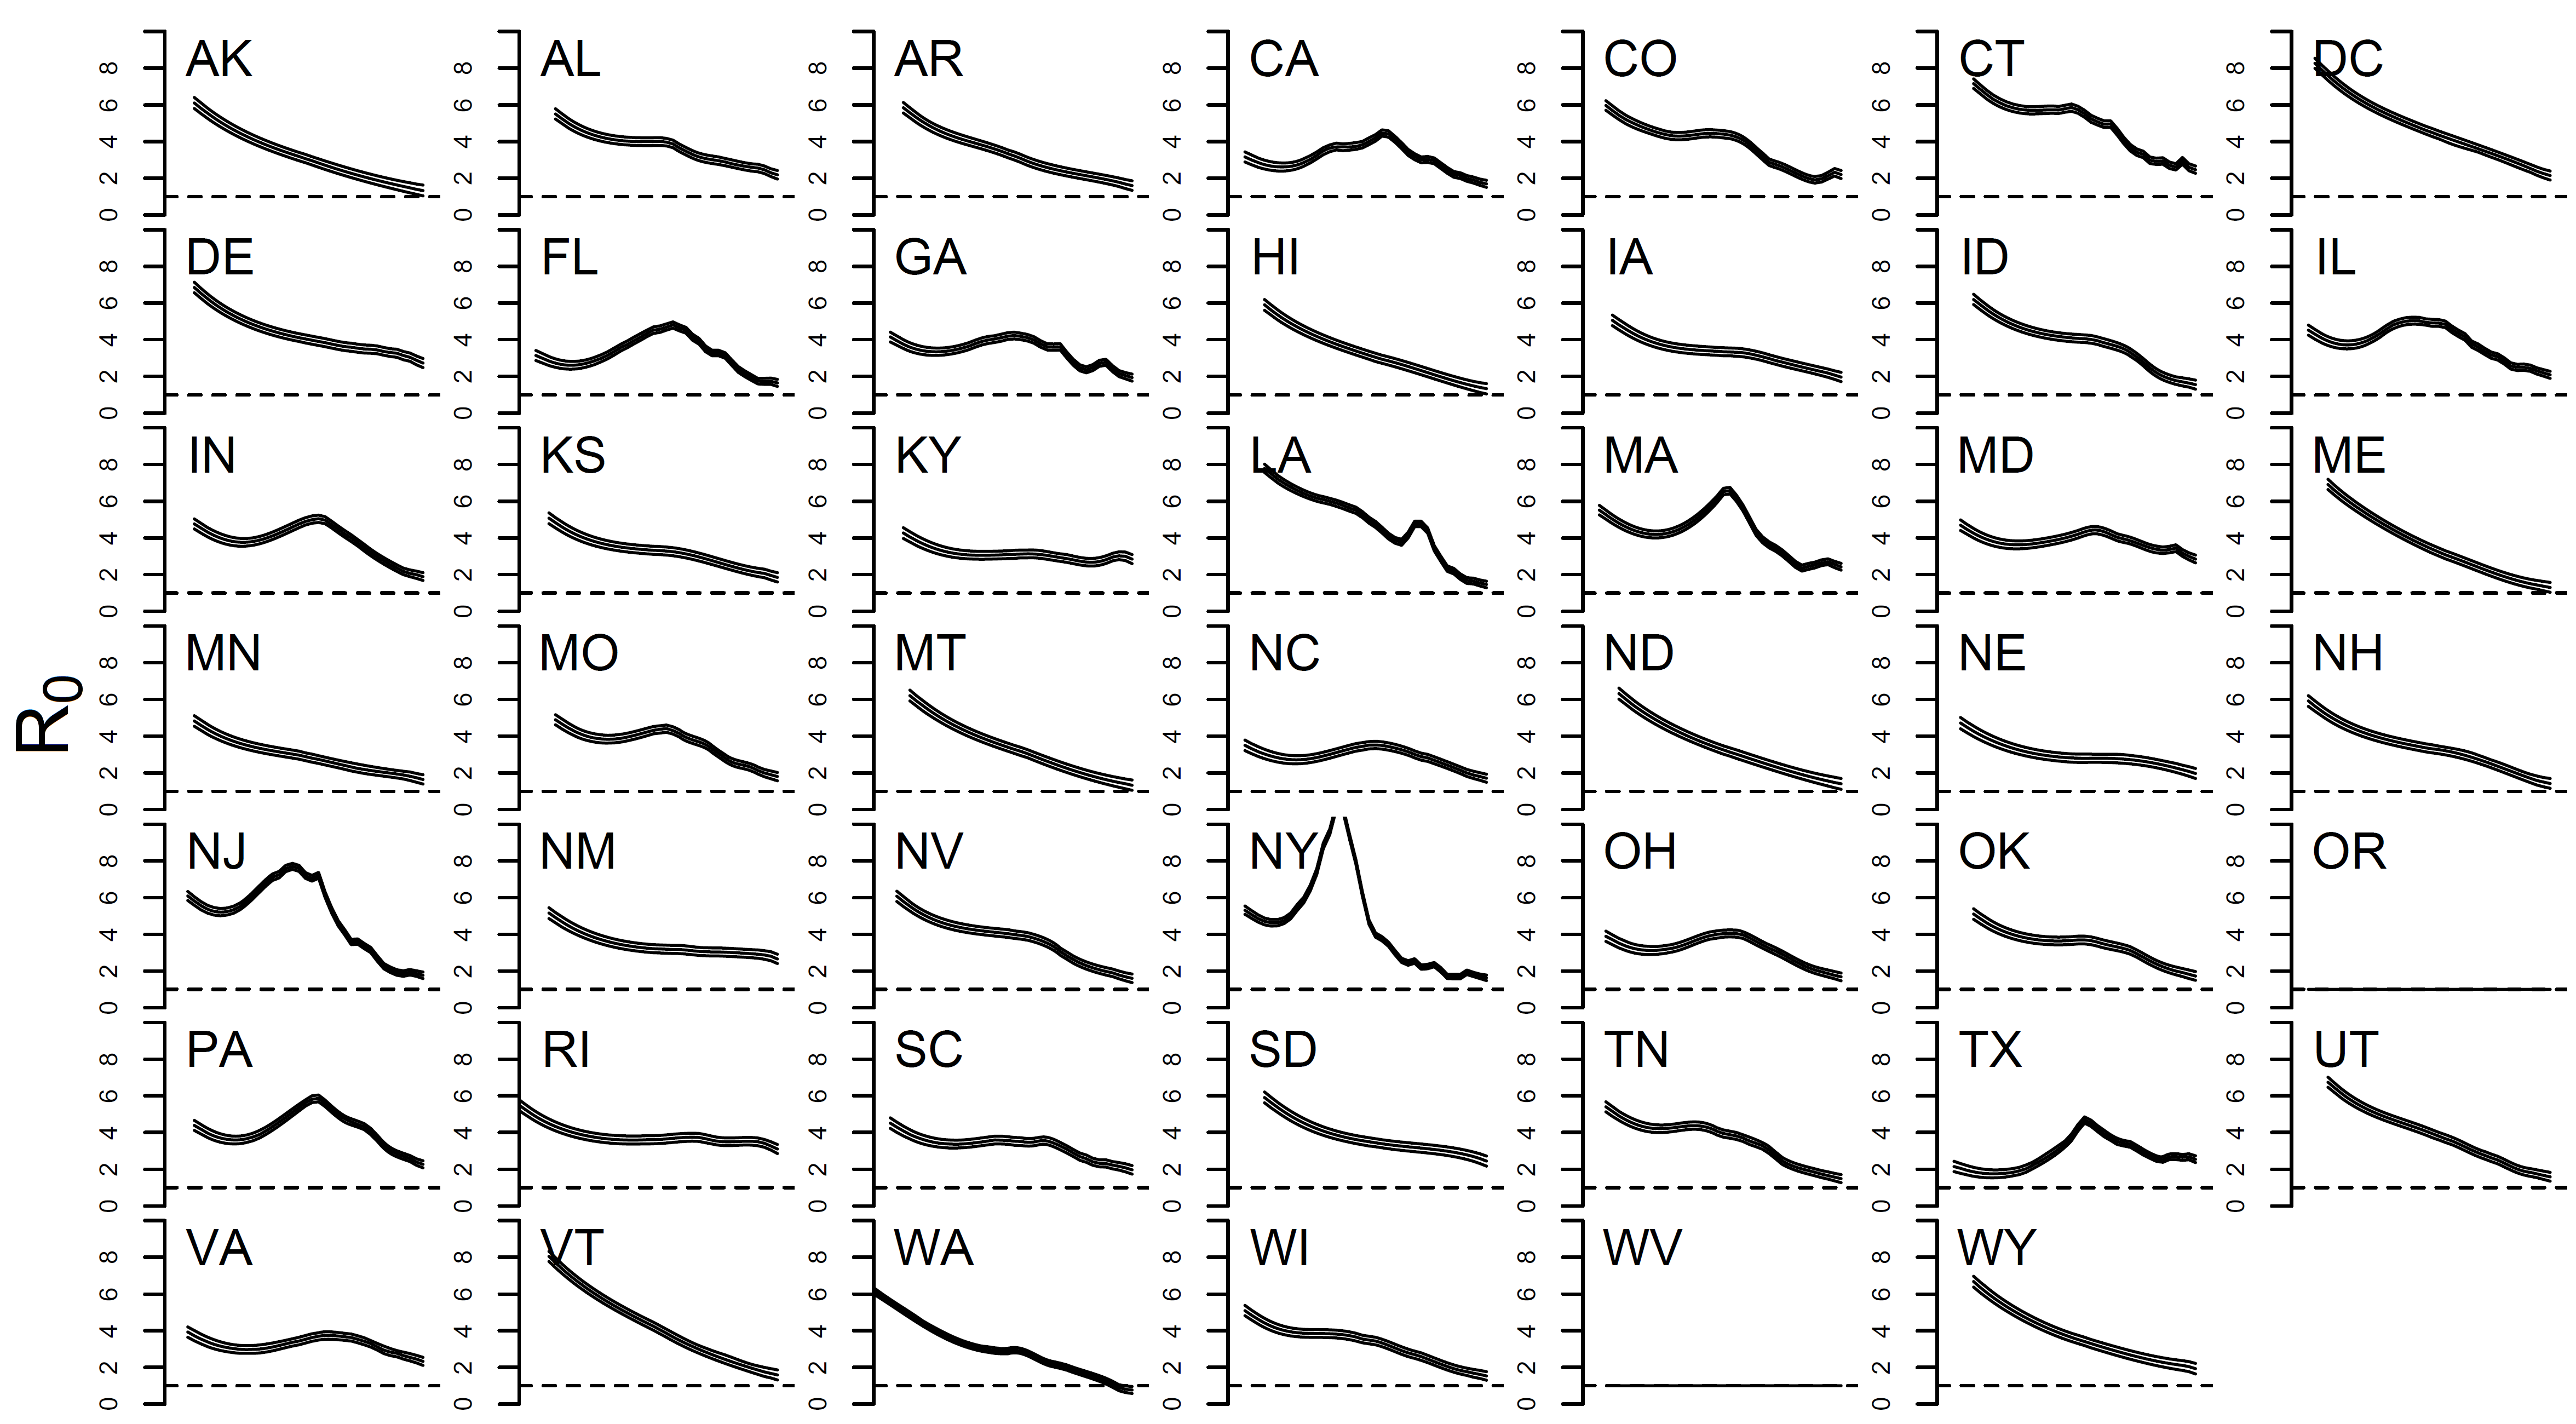
\includegraphics[width=18cm]{beta_AR1_fits_R0.png}
\caption{}
\label{fig:bends}
\end{figure} 
\begin{figure}


\centering
\hspace*{0cm}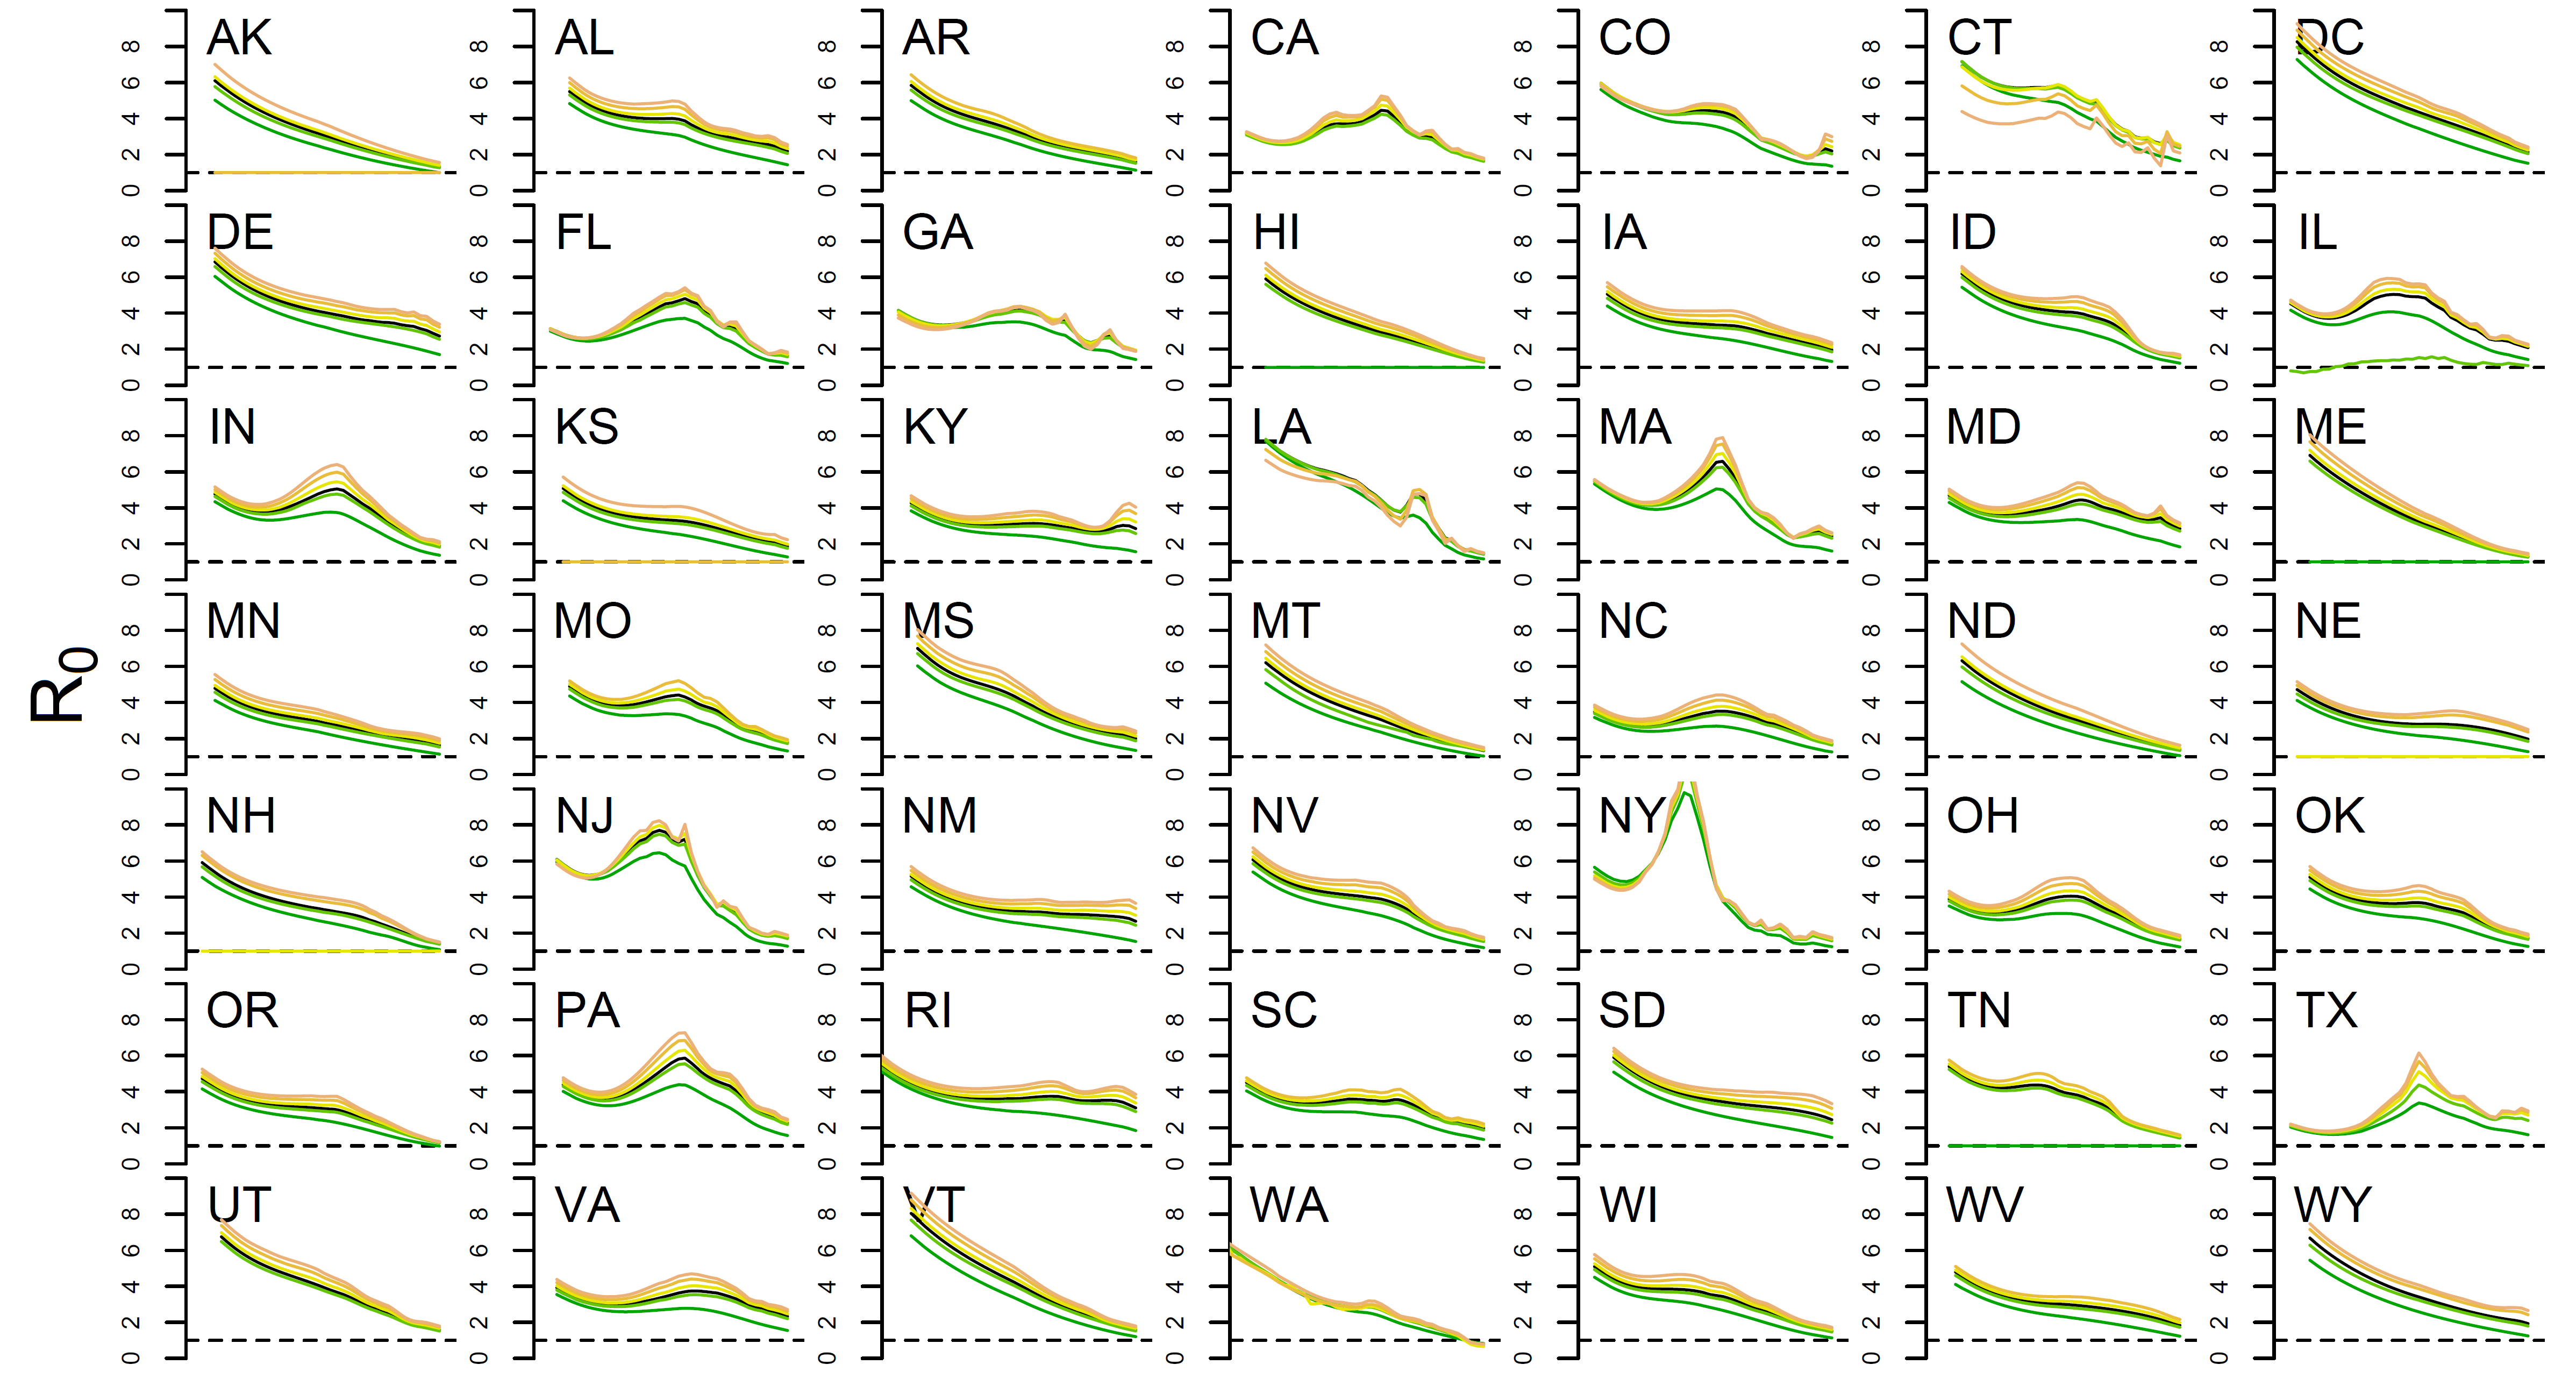
\includegraphics[width=18cm]{beta_AR1_fits_R0_ps_sensitivity.png}
\caption{}
\label{fig:bends}
\end{figure} 
%%%%%%%%%%%%%%%%%%%%%%%%%%%%%%%%%%%%%%%%%%%%%%%%%%%%%%%%%%%%%%%%%%%%%%%%%%%%%%%%%%%%
%% DISCUSSION %%%%%%%%%%%%%%%%%%%%%%%%%%%%%%%%%%%%%%%%%%%%%%%%%%%%%%%%%%%%%%%%%%%%%%
%%%%%%%%%%%%%%%%%%%%%%%%%%%%%%%%%%%%%%%%%%%%%%%%%%%%%%%%%%%%%%%%%%%%%%%%%%%%%%%%%%%%
\section*{Discussion}

%%%%%%%%%%%%%%%%%%%%%%%%%%%%%%%%%%%%%%%%%%%%%%%%%%%%%%%%%%%%%%%%%%%%%%%%%%%%%%%%%%%%
%% Bibliography %%%%%%%%%%%%%%%%%%%%%%%%%%%%%%%%%%%%%%%%%%%%%%%%%%%%%%%%%%%%%%%%%%%%
%%%%%%%%%%%%%%%%%%%%%%%%%%%%%%%%%%%%%%%%%%%%%%%%%%%%%%%%%%%%%%%%%%%%%%%%%%%%%%%%%%%%
%\bibliography{Mendeley}

%%%%%%%%%%%%%%%%%%%%%%%%%%%%%%%%%%%%%%%%%%%%%%%%%%%%%%%%%%%%%%%%%%%%%%%%%%%%%%%%%%%%%
%%%%%%%%%%%%%%%%%%%%%%%%%%%%%%%%%%%%%%%%%%%%%%%%%%%%%%%%%%%%%%%%%%%%%%%%%%%%%%%%%%%%%
%%%%%%%%%%%%%%%%%%%%%%%%%%%%%%%%%%%%%%%%%%%%%%%%%%%%%%%%%%%%%%%%%%%%%%%%%%%%%%%%%%%%%
\end{document}